\documentclass[11pt,a4paper]{article}
\usepackage[utf8]{inputenc}
\usepackage[T1]{fontenc}
\usepackage{amsmath}
\usepackage{bigstrut}
\usepackage{amsfonts}
\usepackage[dvipsnames,table,xcdraw]{xcolor}
\usepackage{amssymb}
\usepackage{caption}
\usepackage{hyperref}
\usepackage{titlesec}
\usepackage{multirow}
\usepackage{subcaption}
\usepackage{wrapfig}
\usepackage{lscape}
\usepackage{rotating}
\usepackage[spanish]{babel}
\usepackage[section]{placeins}
\usepackage{tablefootnote}
\usepackage{graphicx}
\usepackage{epstopdf}
\usepackage[font=scriptsize,labelfont=bf]{caption}
\usepackage{anysize}
\marginsize{3cm}{3cm}{2.5cm}{2.5cm}
\providecommand{\abs}[1]{\lvert#1\rvert}
\providecommand{\norm}[1]{\lVert#1\rVert}
\renewcommand{\thesubsection}{\thesection.\alph{subsection}}
\author{Emanuel Alfredo Cortez Médici}
\title{Trabajo Práctico 1}
\DeclareGraphicsExtensions{.jpg,.png}
\usepackage{float}
\usepackage{fancyhdr}
\hypersetup{
    colorlinks,
    linkcolor={red!50!black},
    citecolor={blue!50!black},
    urlcolor={blue!80!black}
}

\urlstyle{same}
\pagestyle{fancy}
\fancyhf{}
%\lhead[\leftmark]{\leftmark}
\rhead[\thepage]{\thepage}

\usepackage{pifont}

\usepackage{soul}
\setstcolor{red}
\setulcolor{red}
\usepackage[tablename=Tabla]{caption}



\begin{document}
	\begin{titlepage}
	\centering
	
	
\includegraphics[width=0.1\textwidth]{fotos_ema/unsl.png} 
	
	{\scshape\LARGE Universidad Nacional de San Luis\par}
	{\scshape Facultad de Ciencias Físico Matemáticas y Naturales.\par}
	{\scshape Ingeniería Electrónica con O.S.D.\par}
	\vspace{1.5cm}
	{\scshape\Large  \par}
	\vspace{1.5cm}
	{\huge\bfseries  Proyecto de diseño y cálculo de una sección de red de telecomunicaciones apta para brindar servicios triple play. \par}

	\vspace{2cm}
	Alumnos\par
	{\Large\itshape Delle Donne Julián \par 
	Toranzo Deivi \par 
	Cortez Médici Emanuel\par}
	\vfill
	Profesores Responsables\par
	Ing. Alfredo ~\textsc{Debattista}\\
	Ing. Sergio ~\textsc{Hernandez} \\
	Ing. Marwan ~\textsc{Geraiges}
	
	\vfill

% Bottom of the page
	{\large \today\par}
\end{titlepage}

\newpage

\tableofcontents

\clearpage
\part{Introducción}

El presente proyecto pretende analizar y diseñar una red de telecomunicaciones capaz de brindar un servicio de triple play en la localidad de  Leandro N. Alem, presente en el noreste de la provincia de San Luis, Argentina. El proveedor se encuentra en la localidad de Quines de la provincia de San Luis.

Se denomina Triple Play al paquete conjunto de servicios de conexión telefónica, televisiva y a Internet. El servicio Triple Play es un término de marketing que utilizan los operadores de telecomunicaciones para ofertar, a través de una única conexión de banda ancha, tres servicios como son acceso a Internet de banda ancha, televisión y teléfono fijo.

Para poder brindar el servicio, teniendo en cuenta la distancia entre las dos localidades, se necesita implementar dos redes: una red de transporte, que unirá ambas localidades, y una red de acceso, que se encargará de distribuir el servicio dentro de la localidad de Leandro N. Alem.

En el análisis se evaluarán aspectos técnicos, socioeconómicos y geográficos, considerando:

\begin{itemize}
    \item topografía y climatología de la zona
    \item situación socioeconómica de la zona
    \item actividad productiva principal y distribución etaria
    \item servicios existentes y competidores
    \item instalación y mantenimiento de los equipos
    \item penetración del servicio y costos de instalación
\end{itemize}

Una vez realizado el estudio se podrá determinar la mejor solución en cuanto al trayecto del enlace, distribución del servicio, flujo de datos, equipamiento necesario, infraestructura e inversión a realizar para poder por último determinar la rentabilidad del proyecto.

\clearpage
\part{Análisis demográfico y socioeconómico}

\section{Departamento de Ayacucho}
Tiene 9.681 km$^2$ y limita al este con los departamentos de Junín y San Martín, al sur con los de Coronel Pringles y Belgrano, al oeste con las provincias de Mendoza y San Juan, y al norte con las de San Juan, La Rioja y Córdoba, lo que lo convierte en el único departamento de la Argentina que limita con cuatro provincias.

\section{Localidad de Leandro N. Alem.}

Leandro N. Alem es una localidad del departamento Ayacucho, en el norte de la provincia de San Luis, Argentina, situada a 110 kilómetros de la ciudad capital de San Luis.


\section{Análisis demográfico}
Según el censo del Instituto Nacional de Estadísticas y Censos (I.N.D.E.C.) del año 2010, el departamento de Ayacucho presenta una población total de 19.613 habitantes. De este departamento se desea analizar particularmente la localidad de Leandro N. Alem, ya que en esta se pretende brindar el servicio. De dicho censo, se obtuvo que la localidad de Leandro N. Alem contaba en el año 2.010 con 379 habitantes, lo que representa un incremento del 30$\%$ frente a los 291 habitantes censados con el censo anterior.

Debido a que se necesita un análisis actual de la situación poblacional de la localidad, se presentará en cada tabla una estimación al actual año 2.021. Para ello, se utilizará una proyección poblacional estimada del departamento de Ayacucho, realizada por la Dirección Provincial de Estadísticas y Censos de la provincia de San Luis. En la misma, se indica que la población total para julio de 2.021 será de 22.266 habitantes. Para estimar la población presente en julio del año 2.021 en la localidad de Leandro N. Além se tuvo en consideración el porcentaje de personas que representaba dicha localidad respecto del departamento de Ayacucho teniendo en cuenta el censo del año 2.010.

Para entonces, Leandro N. Alem representaba el 1,93$\%$ de la población total del departamento Ayacucho. 
Esta conclusión se obtiene de la ecuación \ref{eq:porc_alem}.

\begin{equation}
    \frac{\text{Población de Leandro N. Alem en el año 2.001}}{\text{Población del departamento Ayacucho en el año 2.001}}*100\%=\frac{379}{19613}*100\%=1.93\%
    \label{eq:porc_alem}
\end{equation}

Contrastando con lo que sucedía en el año 2001, se observa que la población de Leandro N. Alem en aquel año representaba el 1,72\% del departamento de Ayacucho,
por lo tanto se puede estimar la población actual utilizando el porcentaje calculado del año 2010, ya que no se percibe una variación importante entre décadas. 
Teniendo en cuenta que la población correspondiente al año 2.021 para el departamento de Ayacucho es de 22.266 personas y suponiendo que se mantuvo constante el porcentaje de la población que reside en Leandro N. Alem, la cantidad de personas estimada para el año 2.021 es de 430 personas. 
Gracias a declaraciones de la intendencia, se pudieron corroborar estas suposiciones. 
Estos resultados se presentan en la tabla \ref{tab:habitantes_futur_alem}.

\begin{table}[htbp]
 \resizebox{\textwidth}{!}{%
  \centering
  
    \begin{tabular}{|c|p{0.25\linewidth}|p{0.25\linewidth}|p{0.25\linewidth}|}
    \hline
    Lugar & Cantidad de habitantes para el año 2.001 & Cantidad de habitantes para el año 2.001 & Cantidad de habitantes para el año 2.021 \\
    \hline
    Ayacucho & 16906 & 19613 & 22266 \\
    \hline
    Leandro N. Alem & 291  & 379  & 430 \\
    \hline
    \end{tabular}}%
    \caption{cantidad de habitantes en el año 2.010 y previstos para julio del 2.021 en la localidad de Leandro N. Alem.}
  \label{tab:habitantes_futur_alem}%
\end{table}%


Gracias a los datos aportados por el censo del I.N.D.E.C. y la estimación de la Dirección Provincial de Estadísticas y Censos de la Provincia de San Luis, se pueden analizar la cantidad de hogares con necesidades básicas insatisfechas en ambas localidades y la cantidad de personas por hogar.

Por otro lado, el I.N.D.E.C. brinda además información sobre la cantidad de usuarios que poseen computadoras, teléfonos fijos y teléfonos celulares. 
Dicha información se presenta en la Tabla 5.
Esta información es de particular interés, ya que es necesaria para determinar los posibles usuarios del servicio que se desea brindar.
Se presenta juntamente, una cantidad actual supuesta.
Para ello, se utilizaron los datos brindados por el I.N.D.E.C., los cuales mostraban que al cuarto trimestre del año 2019, el 79,9$\%$ de la población argentina tenía acceso a internet.
Además, entre el cuarto trimestre de 2019 y el cuarto trimestre de 2020, se produjo un crecimiento interanual en la utilización de internet del 1,1$\%$.
Por lo tanto, esto resulta en que el 80,78$\%$ de la población utiliza actualmente internet.
Debido a que se necesitan de estos dispositivos para acceder a internet, es que se puede suponer que la cantidad de los mismos aumentó en la misma proporción.

Los datos recabados y previstos son mostrados en la tabla \ref{tab:prediccion_alem}.


\begin{table}[htbp]
  \centering
    \begin{tabular}{|p{0.45\linewidth}|c|c|}
    \hline
    Localidad & \multicolumn{2}{|c|}{Leandro N. Alem} \\
    \hline
    Año  & 2010 & Previsión 2021 \\
    \hline
    Población & 379  & 430 \\
    \hline
    Población con necesidades básicas insatisfechas & 12   & 14 \\
    \hline
    Cantidad de personas por hogar & 3    & 3 \\
    \hline
    Cantidad de personas que poseen computadoras, teléfonos fijos o teléfonos celulares & 132  & 347 \\
    \hline
    \end{tabular}%
    \caption{análisis demográfico en la localidad de Leandro N. Alem.}
  \label{tab:prediccion_alem}%
\end{table}%


Una vez definidos los distintos habitantes y hogares que pueden satisfacer sus necesidades básicas, es necesario agrupar aquellos que poseen características en común para así poder determinar los tipos de servicios que se pueden brindar.

Una característica importante para determinar el modelo de consumo, es la edad.
Dependiendo de la edad, existirán o no requerimientos mayores en el servicio de internet y/o televisión.
Por dicho motivo se analizarán 3 grupos etarios, personas entre 25 y 35 años, personas entre 35 y 60 años y personas mayores de 60 años. 
Esta elección en la división se realizó teniendo en cuenta características en común en dichas franjas etarias, siendo todas personas que generalmente están en edad de trabajar o de recibir un sueldo, si es que los mismos son jubilados.

Para la edad entre 25 y 35 años, se encontró que en el 2.001 existían en Leandro N. Alem 20 personas en dicho rango etario, representando el 6,9$\%$ del total. 
Para el año 2.010, esta cantidad aumentó a 48 personas, representando el 12,7$\%$ del total.
Debido a la gran variabilidad en la composición etaria que suelen presentar los pueblos, es que a pesar del aumento abrupto en la proporción a lo largo del periodo 2.001-2.010, es que se decide utilizar el porcentaje obtenido con el censo del año 2.010 y trasladarlo al año 2.021 sin aumentarlo.
Realizando esto, se estima que existen 55 personas entre 25 y 35 años.

Para la edad entre 35 y 60 años, se encontró que en el 2.001 existían 88 personas en dicho rango etario, los cuales conformaban el 30,2\% de la población total. En el año 2.010, existían 105 personas, conformando el 27,7\% del total.
Debido a que la variación no fue significativa en el periodo entre décadas, se utiliza el mismo porcentaje que el obtenido para el año 2.010. 
Con dicha consideración, se estima que en la actualidad existen 119 personas pertenecientes a dicho rango etario.

Finalmente, para el grupo etario de mayores de 60 años, se obtuvo que en el año 2.001 existían 70 habitantes, representando el 24$\%$ del total poblacional, mientras que en el año 2.010 existían 79 personas, representando el 20,8$\%$. A pesar de la reducción en este grupo, se prefiere continuar con este porcentaje para la estimación del año 2.021.
Con el porcentaje mencionado, se obtuvo que existen en Leandro N. Alem 89 habitantes mayores a 60 años.
Los datos previamente calculados se muestran en la tabla \ref{tab:etario_alem}.

Con dichos datos, se podrán determinar distintos grupos a los cuales brindar un servicio adecuado a sus necesidades e intereses.



\begin{table}[htbp]
  \centering
    \begin{tabular}{|p{0.3\linewidth}|c|c|}
    \hline
    Localidad & \multicolumn{2}{|c|}{Leandro N. Alem} \\
    \hline
    Año  & 2010 & Previsión 2021 \\
    \hline
    Personas entre 25 y 35 años & 20   & 48 \\
    \hline
    Personas entre 35 y 60 años & 88   & 105 \\
    \hline
    Personas mayores a 60 años & 70   & 79 \\
    \hline
    \end{tabular}%
  \caption{análisis de los distintos grupos etarios en la localidad de Leandro N. Alem.}
  \label{tab:etario_alem}%
\end{table}%

\section{Análisis económico}

Observando la Fig. \ref{fig:agropecuaria} y la Fig. \ref{fig:industria}, se puede concluir que la principal actividad privada que se desarrolla en el departamento Ayacucho es la actividad agropecuaria.

\begin{figure}[ht!]
  \centering
  \subcaptionbox{actividad agropecuaria por departamento.\label{fig:agropecuaria}}%
  [.45\linewidth]{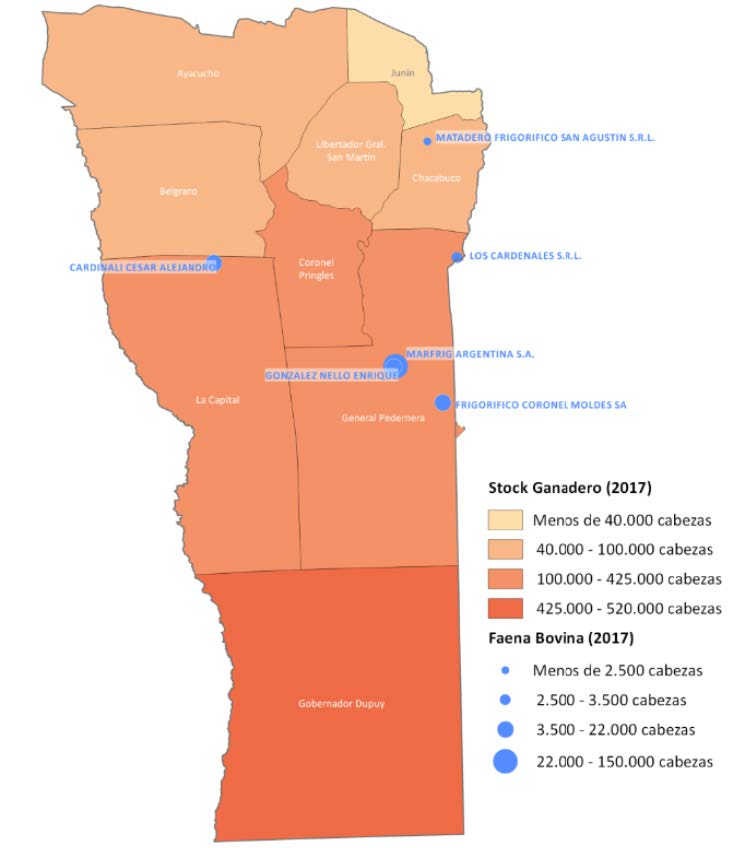
\includegraphics[height=15\baselineskip]{fotos_ema/agropecuaria}}
\subcaptionbox{actividad industrial por departamento.\label{fig:industria}}
  [.45\linewidth]{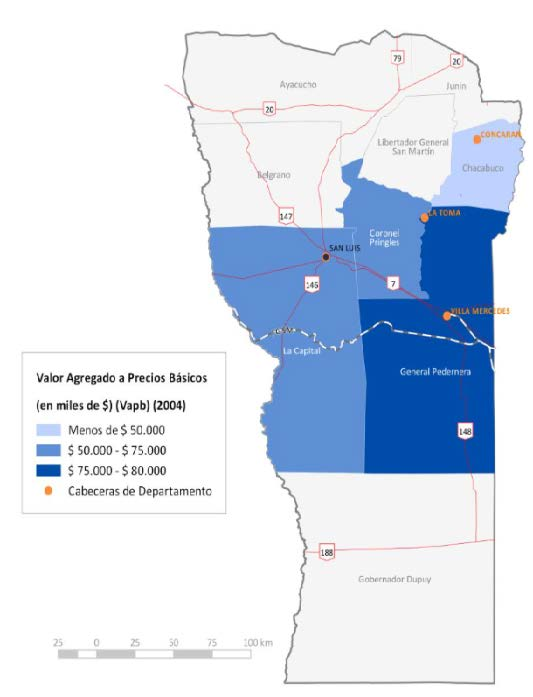
\includegraphics[height=15\baselineskip]{fotos_ema/industria}}
  \caption{actividades económicas de la provincia de San Luis por departamento.}
  \label{fig:econo_deptos}
\end{figure}

Por lo tanto, si se tienen en cuenta los datos aportados por la tabla \ref{tab:salarios_alem}, para el año 2.017 se tiene un sueldo de \$17.691. 
Tomando en cuenta que la inflación acumulada en los años 2.017, 2.018, 2.019 y 2.020 es del 162,3\%, se puede determinar que el valor actual ajustado por inflación corresponde a \$46.403 pesos argentinos para el sector privado.

Por otro lado, el sector público, el cual representa el 16\% de la población total, y el 35,5\% de la población laboralmente activa, poseía al año 2017 un sueldo promedio de \$24.172. 
Teniendo en cuenta la inflación acumulada mencionada anteriormente, se puede determinar que el valor actual ajustado por inflación corresponde a \$63.403 pesos argentinos para el sector público.

Finalmente, se puede determinar que el sueldo promedio general que se considerará será de \$52.470. Esto se obtuvo de la ecuación \ref{eq:sueldo_promedio_alem}.


\begin{equation}
    \$63403*35.5\% + \$46403*64.5=\%52.470
    \label{eq:sueldo_promedio_alem}
\end{equation}


Tomando en cuenta la cantidad de personas por hogar, mostradas en la Tabla 4, se puede determinar un grupo familiar formado por 1 matrimonio y 1 hijo, el cual puede presentar como ingreso un sueldo general, previamente desarrollado.
La ventaja de considerar este tipo de grupo con una sola fuente de ingreso es que puede nuclear también una familia monoparental.
Debido a que este grupo incluye un ingreso el cual puede ser proveniente tanto del sector público o privado, se puede suponer que este representa el 50\% de la población laboralmente activa, es decir la población entre 25 y 60 años.
Considerando esto, este grupo representa el 33,1\% de la población que recibe un ingreso.
Otro grupo a considerar es un matrimonio de jubilados, suponiendo que ambos cobran la jubilación mínima, esto da un ingreso total de \$41.142. 
Del análisis anterior se puede suponer que este grupo representa el 20,7\% de la población total, y el 33,8\% de la población que percibe un ingreso, analizada previamente. 
Un tercer grupo familiar a tener en cuenta es el conformado por 2 fuentes de ingreso, suponiendo que una proviene de trabajar en el sector privado y otra de trabajar en el sector público. 
Esto da un ingreso total de \$109.806.
Debido a lo analizado previamente, la proporción de este grupo se puede estimar teniendo en cuenta el porcentaje restante de la población que percibe un ingreso, dando cómo resultado una proporción del 33,1\%. Estos datos se presentan en la tabla \ref{tab:grupos_sueldos_alem}.


\begin{table}[htbp]
  \resizebox{\textwidth}{!}{%
  \centering
    \begin{tabular}{|p{0.25\linewidth}|p{0.25\linewidth}|p{0.25\linewidth}|p{0.25\linewidth}|}
    \hline
    Sector & Rama de actividad & Salario en pesos promedio en el año 2.017 & Salario en pesos previsto para el año 2021 \\
    \hline
    Privado & Agricultura, ganadería y pesca & \$17.691 & \$46.403 \\
    \hline
    Público & Servicios & \$24.172 & \$63.403 \\
    \hline
    \end{tabular}}%
      \caption{salario en pesos promedio en 2.017 y previsto para 2.021.}
  \label{tab:salarios_alem}%
\end{table}%




\begin{table}[htbp]
  \resizebox{\textwidth}{!}{%
  \centering
    \begin{tabular}{|p{0.3\linewidth}|p{0.3\linewidth}|p{0.3\linewidth}|}
    \hline
    Grupos & Sueldo considerado & Porcentaje aproximado de la población que percibe un ingreso \\
    \hline
    Grupo familiar con una sola fuente de ingreso & \$ 52.470 & 33,10\% \\
    \hline
    Jubilados & \$ 41.142 & 33,80\% \\
    \hline
    Grupo familiar con dos fuentes de ingreso & \$ 109.806 & 33,10\% \\
    \hline
    \end{tabular}}%
  \caption{resumen de los distintos grupos económicos.}
  \label{tab:grupos_sueldos_alem}%
\end{table}%


Un indicador fundamental para determinar el porcentaje de la población que podrá acceder a nuestros servicios fue el de Necesidades Básicas Insatisfechas (N.B.I.). 
El mismo permite identificar características críticas en la población y delimitar grupos de pobreza que no tienen los ingresos suficientes para pagar nuestro servicio. 
Según las estadísticas mostradas en la Tabla 3 , se registraron 12 personas con NBI en la localidad de Leandro N. Alem en el año 2.010, representando el 3,16\% de la población total.

Haciendo uso de la proyección poblacional estimadas anteriormente al año 2.021 y teniendo en cuenta que las siguientes consideraciones quedan excluidas del razonamiento:

\begin{itemize}
    \item La pandemia causada por el COVID 19
    \item La tasa inflacionaria del país
    \item Las diversas crisis económicas que atravesó el país
    \item Corrida cambiaria y desestímulo a la inversión privada
\end{itemize}

Se puede realizar entonces una estimación del índice de NBI que presenta la localidad en la actualidad, considerando que este se mantiene constante a lo largo de la década. 
Esto da como resultado un total de 14 personas con NBI. 
Si bien esta no es la mejor aproximación, se optó por utilizarla de referencia dado que no se pudo encontrar información actualizada sobre este índice.

En la tabla 4 se puede observar la cantidad promedio de personas por hogar que había en el año 2.010, siendo esta de 3 personas. 
Si consideramos que en la actualidad el promedio de personas por hogar sigue siendo el mismo, y teniendo en cuenta que la población total estimada para el año 2.021 fue de 430 habitantes, se puede calcular la cantidad de hogares a partir de la ecuación \ref{eq:hogares_alem}, dando como resultado 144 hogares.

\begin{equation}
    \frac{\text{Población de Leandro N. Alem en el año 2.021}}{\text{Cantidad de personas por hogar}}=\frac{430}{3}=144
    \label{eq:hogares_alem}
\end{equation}


Siguiendo el mismo razonamiento descrito anteriormente se puede calcular la cantidad de hogares con NBI en la localidad de Leandro N. Além, dando como resultado un total de 5 hogares con NBI. Debido a que no pueden cubrir sus necesidades básicas, lamentablemente no se podrán considerar en la prestación del servicio. 
Esto deja disponible la cantidad de 139 hogares para brindar el servicio.

\section{Análisis competitivo}

Debido a que la provincia de San Luis cuenta con antenas Wi-Fi públicas, es menester analizar si estás proveen de buen internet a la zona o si el servicio está saturado. 
Sin embargo, haciendo uso del sitio web nperf.com, se puede corroborar que en esta localidad no se encuentran antenas de ningún proveedor de telefonía móvil (Claro, Personal o Movistar) lo que favorece a la hora de buscar posibles consumidores. 
Por otro lado, cabe destacar la inexistencia de proveedores de televisión por cable. 
El servicio de TV llega solamente a través de la empresa DirecTV. 
Por lo tanto, se procederá a realizar un relevamiento tanto del servicio de internet brindado por el estado, así como los posibles precios que maneja DirecTV.


\subsection{Wi-Fi público}

En la localidad de Leandro N. Alem, se encuentran presentes 4 antenas Wi-Fi, tal como se observa en la Fig. 3.
De estas 4 antenas, 3 trabajan con una frecuencia de 2,4 GHz, mientras que sólo una trabaja con 5 GHz.
Analizando el uso de las antenas en horarios picos, se obtuvo un promedio de 34 usuarios por antena.
Considerando el tipo de antena predominante y la cantidad de usuarios por antena, se puede concluir que, efectivamente, el servicio de internet público se encuentra saturado, prestando la oportunidad de brindar una alternativa de pago que ofrezca un mejor comportamiento.

\subsection{DirecTV}

Debido a la falta de televisión por cable, la televisión satelital es la única opción con la que disponen los habitantes de Leandro N. Alem, siendo la opción de pago más extendida en Argentina DirecTV. 
Observando los precios en la página oficial de DirecTV, se tiene que el servicio básico tiene un precio de \$2.098, con 145 canales HD, mientras que el mejor servicio posee un precio de \$3.393, con 255 canales HD 4K.
Es por ello, que al analizar los precios que se desearán manejar, se deberá respetar este margen de precios.
No obstante, a pesar de la gran oferta brindada por este servicio, un talón de Aquiles presente es la inestabilidad del servicio ante las inclemencias del tiempo, tales como vientos, muy presentes en la zona, o lluvias.
Esto deja margen a que, si se puede brindar un servicio que sea estable, incluso con una oferta menor, se pueda competir fácilmente con el prestador dominante.

\subsection{Características del servicio que se desea brindar}

Mediante el análisis demográfico, se deduce que la mayor parte de Leandro N. Alem es zona rural.
Por lo tanto, se deben tener en cuenta las posibles necesidades de una persona de campo, como por ejemplo: el diario/ agencia de noticias, el canal del clima, canal “La rural”, etc. 
El servicio de Wi-Fi público en hora pico hace imposible el uso de estos sitios web, por lo tanto se debe proveer un servicio con ancho de banda capaz de satisfacer estas necesidades. 
Lo mismo ocurre con el servicio de televisión de Directv en los días de lluvia o vientos fuertes.
Además de poseer un catálogo de canales innecesariamente grande para este tipo de consumidores por lo que se dispondrá tener una cantidad reducida de canales (que contengan los canales anteriormente nombrados).
Luego de los distintos análisis realizados, se procederá a determinar las características del servicio que se pretende brindar en la zona.

\subsection{Televisión}

Se ofrecerán 2 servicios, uno básico con 50 canales SDTV y otro premium con 56 canales, 6 de los cuales serán HDTV y 50 SDTV. 
Se toman 6 canales HD, para cubrir la necesidad de ver canales de deportes y películas en una mejor resolución.

\subsection{Internet}

Junto con el servicio básico, se ofrecerán 6 mbps, mientras que el servicio premium contará con una velocidad de 15 mbps.

\subsection{Precio, contenido y alcance del servicio}

Con el desarrollo del análisis económico, se llega a que el salario promedio de un habitante de Leandro N. Alem es de \$52.470.
Para poder abrirse paso entre la competencia, se considera no cobrar más del 8\% del salario promedio, lo que da un límite de \$4.197.
Además, para no abrumar a los posibles clientes con tantas posibilidades, se pone a disposición solo tres opciones. 
Por lo tanto, los precios de nuestro servicio y su contenido son los mostrados en la tabla \ref{tab:precios}. 
El pack básico que cuenta con un servicio de 50 canales SDTV está pensado para el grupo etario de mayores a 60 años, que según el estudio realizado anteriormente, está conformado por alrededor de 89 personas. 
El pack intermedio tiene como objetivo a familias con uno o dos salarios básicos que quieran acceder a un servicio de internet decente contando además con el servicio de 50 SDTV. 
Por último, el pack premium está destinado a personas con un salario mayor al promedio y quieren adquirir un servicio de internet y televisión de buena calidad.
Al ser este un sector más reducido se estima que será el pack que menos se contrate.


\begin{table}[htbp]
  \centering
    \begin{tabular}{|c|c|c|}
    \hline
    Tipo de pack & Contenido & Precio en pesos \\
    \hline
    Básico & 50 SDTV & \$1500 \\
    \hline
    Intermedio & 50 SDTV+6 mbps &  \$2800 \\
    \hline
    Premium & 50 SDTV+6 HDTV+15 mbps & \$4000 \\
    \hline
    \end{tabular}%
  \caption{precios del servicio}
  \label{tab:precios}%
\end{table}%



Considerando que los hogares con N.B.I harán uso del Wi-fi público y que no todos los habitantes van a querer adquirir alguno de los packs propuestos ya que un porcentaje de la población optará por continuar usando la red pública y aprovechar la migración de usuarios a este nuevo servicio, esto ocasionará un alivio en la red, convirtiéndola en una red utilizable si solo se conecta un 40\% (alrededor de 41 personas por antena) de la población tenida en cuenta para los análisis previos.
Por otro lado, el porcentaje de la población que es cliente de DirecTV optará por adquirir este nuevo servicio al tener un precio menor y mayor fiabilidad frente a los cambios climáticos.
Por lo tanto, el porcentaje de población que adquirirá este servicio es del 60\%, dando un total de 83 hogares.



\section{Modelo de consumo}

Del estudio socioeconómico realizado se obtuvo como conclusión que 83 hogares del total de la población de la localidad de Leandro N. Alem serían potenciales clientes. 
En base a este resultado se procede a calcular el ancho de banda total de cada servicio proporcionado y en consecuencia el ancho de banda total que deberá soportar la red troncal.

\subsection{TV}

En la tabla \ref{tab:tv_maxima} se observa la máxima cantidad simultánea para cada tipo de servicio que se ofrece y su correspondiente ancho de banda. Multiplicando la mayor cantidad de canales de cada tipo (SDTV y HDTV) por su correspondiente ancho de banda se obtiene la tasa de bit necesaria para la transmisión del servicio de TV.
Esto se muestra en la ecuación \ref{eq:tasa_bits_tv}.

\begin{equation}
    \text{Tasa de bits: } 50*1.5*10^6+6*6*10^6=111 \text{ Mbps}
    \label{eq:tasa_bits_tv}
\end{equation}

No se considera necesaria la utilización de buffer ya que se transmitirán solo 56 canales.

\begin{table}[htbp]
  \centering
    \begin{tabular}{|c|c|c|}
        \hline 
        \textbf{Servicio} & \textbf{Ancho de banda} & \textbf{Cantidad Máx. simultánea} \\ \hline 
        \textbf{Canal SDTV} & 1.5 Mbps & 50 \\ \hline 
        \textbf{Canal HDTV} & 6 Mbps & 6 \\ \hline 
        \textbf{VoIP} & 30 kbps & 83 \\ \hline 
        \textbf{Internet} & 6/15 Mbps & 44/14 \\ \hline 
    \end{tabular}
  \caption{Cantidad máxima simultánea vs. ancho de banda}
  \label{tab:tv_maxima}%
\end{table}%


\subsection{VoIP}

La mayor cantidad de clientes que pueden estar usando nuestro servicio es igual a la cantidad de hogares, multiplicando por el ancho de banda que muestra la tabla \ref{tab:tv_maxima} se obtiene un total de 1,92 Mbps. Esto se muestra en la ecuación \ref{eq:tasa_bits_tel}.

\begin{equation}
    \text{Tasa de bits: } 83*30*10^3=1.92 \text{ Mbps}
    \label{eq:tasa_bits_tel}
\end{equation}

Se puede observar que la tasa de bit correspondiente a la transmisión del servicio VoIP es mucho menor al de TV siendo este despreciable a la hora de considerar el ancho de banda total que deberá soportar la red troncal .

\subsection{Internet}
Con los resultados obtenidos previamente se hicieron estimaciones de cuántas personas podrían optar por contratar los pack intermedios y premium que prestan un servicios de 6 y 15 Mbps respectivamente. 
Se consideró realizar un porcentaje de cuántos clientes podrian optar por cada pack en base a su clasificación económica/familiar (familias con uno o dos sueldos y jubilados).
También se consideró la disponibilidad de las antenas de Autopista de la Información que brindan internet en la zona. 
Con este razonamiento en mente se estimaron los resultados de la tabla \ref{tab:porcent_total_packs} donde el 53\% de los 83 posibles clientes optará por el pack intermedio y el 17\% por el pack premium dando como resultado un total de 44 y 14 clientes respectivamente como muestra la tabla \ref{tab:tv_maxima}. 



\begin{table}[htbp]
\resizebox{\textwidth}{!}{%
  \centering
    \begin{tabular}{|c|c|c|c|c|}
    \hline 
    \textbf{Grupo} & \textbf{Pack Básico $[\%]$ } & \textbf{Pack intermedio $[\%]$} & \textbf{Pack premium $[\%]$} & \textbf{Total de grupo $[\%]$} \\ \hline 
    \textbf{Familias con un sueldo} & 4 & 25,1 & 4 & 33.1 \\ \hline 
    \textbf{Familias con dos sueldos} & 2 & 19,1 & 12 & 33.1 \\ \hline 
    \textbf{Jubilados} & 24 & 8,8 & 1 & 33.8 \\ \hline 
    \textbf{Total} & 30 & 53 & 17 & 100 \\ \hline 
    \end{tabular}}
  \caption{porcentaje total de cada grupo que optara por cada uno de los packs.}
  \label{tab:porcent_total_packs}%
\end{table}%


Multiplicando esta cantidad de clientes por el ancho de banda se obtiene la tasa de bit necesaria para el servicio de internet. Esto se muestra en la ecuación \ref{eq:tasa_bits_internet}

\begin{equation}
    \text{Tasa de bits: } 44*6*10^6+14*15*10^6=474 \text{ Mbps}
    \label{eq:tasa_bits_internet}
\end{equation}

 En la tasa de bits correspondiente al utilizado por la red de internet, a diferencia del servicio de TV y VoIP, se considera que no se utiliza el 100\% del ancho de banda. 
 Esto no sucede en la práctica ya que se producen pausas en el tráfico que reducen el uso del ancho de banda. 
 Además, no todos harán uso del servicio de internet al mismo tiempo y en cada caso varía la utilidad que le dan, no siendo lo mismo hacer una videollamada que solo mandar un mensaje de texto o un mail. 
 Teniendo esto en cuenta y además de que Leandro N. Alem es un pueblo pequeño, mayormente agrícola, se considera utilizar un factor de simultaneidad del 30\%.
 Con este factor de simultaneidad se estima poder ofrecer un servicio estable a los usuarios.
 El resultado es una tasa de bits total de 255 Mbps como muestra la ecuación \ref{eq:tasa_de_bits_total}, la cual deberá soportar la red troncal.
 
 \begin{equation}
     \text{Tasa de bits: } 111*10^6+1.92*10^6+142.2*10^6\approx255 \text{ Mbps}
     \label{eq:tasa_de_bits_total}
 \end{equation}


 \clearpage 
\part{Red inalámbrica}



\section{Red troncal con radioenlace}

\subsection{Determinación de las frecuencias a utilizar para la transimisión}

Al analizar los datos disponibles en el sitio web del ENACOM\footnote{\href{https://www.enacom.gob.ar/bandas-de-uso-compartido-sin-autorizacion_p680}{Bandas de uso compartido sin autorización}}, se optará por usar una banda de uso compartido sin autorización ya que dispone de bandas de frecuencias óptimas para la utilización de una antena de 5GHz. 
Las bandas de uso compartido sin autorización se rigen mediante la Resolución del Ministerio de Modernización N$\mathrm{{}^\circ}$ 581/ 18\footnote{\href{https://www.argentina.gob.ar/normativa/nacional/resolución-581-2018-314174}{Resolución del Ministerio de Modernización N$\mathrm{{}^\circ}$ 581/ 18}}, la cual establece que las bandas de frecuencias radioeléctricas, detalladas a continuación en la tabla \ref{tab:frec_libres}, se declaran de uso compartido en el ámbito del territorio nacional y no requieren de autorización para su uso, debiendo respetarse las condiciones y parámetros técnicos de emisión establecidas por el Ente Nacional de Comunicaciones en la Resolución N$\mathrm{{}^\circ}$ 4653/19\footnote{\href{https://www.enacom.gob.ar/multimedia/normativas/2019/res4653.pdf}{Resolución N$\mathrm{{}^\circ}$ 4653/19}}:

\begin{table}[htbp]
  \centering
\begin{tabular}{|c|} \hline 
Rango de frecuencias: \\ \hline 
915-928 [MHz] \\ \hline 
2400-2483.5 [MHz] \\ \hline 
5150-5250 [MHz] \\ \hline 
5250-5350 [MHz] \\ \hline 
5470-5600 [MHz] \\ \hline 
5650-5725 [MHz] \\ \hline 
5725-5850 [MHz] \\ \hline 
57000-71000 [MHz] \\ \hline
\end{tabular}
\caption{rango de frecuencias de uso compartido.}
\label{tab:frec_libres}
\end{table}%


Esto genera un ahorro importante a la hora de calcular costos al no tener que licitar una banda de frecuencias. Asimismo, los usuarios de las bandas de frecuencias de uso compartido que operen en la modalidad de uso \textbf{Prestador} deberán notificar al Ente Nacional de Comunicaciones las coordenadas geográficas, altura de antena de las estaciones radiobases que instalen, datos de homologación del equipo y bandas de frecuencia de operación. Dicha notificación deberá tramitarse a través de la plataforma "Trámites a Distancia" (TAD) del sistema de Gestión Documental Electrónica\footnote{\href{https://tramitesadistancia.gob.ar/}{Trámites a distancia}}. Otro punto importante para hacer uso de esta banda de frecuencia es la potencia permitida. Al analizar la Resolución RESOL-2018-581-APN-MM\footnote{\href{https://www.enacom.gob.ar/multimedia/normativas/2018/res581MM.pdf}{Resolución RESOL-2018-581-APN-MM}} se corrobora que la potencia a utilizar está en el rango permitido.

Con esto definido y con la utilización del CABFRA\footnote{\href{https://www.enacom.gob.ar/cuadro-de-atribucion-de-bandas-de-frecuencias-de-la-republica-argentina-cabfra-\_p1588}{Cuadro de atribución de bandas de frecuencias de la República Argentina}}, el rango de frecuencia desde 5,725 GHz a 5,825 GHz, cuyas características se encuentran en la tabla \ref{tab:rango_frec}, está dentro de los parámetros requeridos. 


\begin{table}[htbp]
\resizebox{\textwidth}{!}{%
  \centering
    \begin{tabular}{|p{0.25\linewidth}|p{0.25\linewidth}|p{0.25\linewidth}|p{0.25\linewidth}|}
    \hline
    \multicolumn{4}{|c|}{Rango de frecuencia} \bigstrut\\
    \hline
    \multicolumn{4}{|c|}{\textbf{5.725 - 5.825}} \bigstrut\\
    \hline
    \multicolumn{4}{|c|}{Observaciones generales} \bigstrut\\
    \hline
    \multicolumn{4}{|c|}{} \bigstrut\\
    \hline
    SERVICIO (T10) & TIPO DE SERVICIO & CARACTERÍSTICAS & NORMATIVA \bigstrut\\
    \hline
    Servicio de Radiolocalización - SRL & FIJO/MOVIL &      & RR UIT/R2 - Art. 5 \bigstrut\\
    \hline
    Servicio de Aficionados - SAF & FIJO/MOVIL & Banda de 5 cm & 3635ENACOM17 508ENACOM18 4653ENACOM19 \bigstrut\\
    \hline
    Servicio TIC para banda de frecuencia de uso compartido & FIJO/MOVIL & Uso Privado - Prestador (5.725 - -5.850 MHZ) & 581MM18 4653ENACOM19 \bigstrut\\
    \hline
    Sistemas de Baja Potencia - SBP & FIJO/MOVIL & Categoría Secundaria (3,1 - 10,6 GHz) & 5186ENACOM17 507ENACOM18 \bigstrut\\
    \hline
    \end{tabular}}%
    \caption{características para el rango de frecuencia entre 5.725 y 5.825 MHz.}
  \label{tab:rango_frec}%
\end{table}%

Para conseguir la canalización de la banda de frecuencias a utilizar, se debe consultar con la tabla de asignación de canales de la frecuencia de 5GHz\footnote{\href{https://www.ekahau.com/blog/channel-planning-best-practices-for-better-wi-fi/}{Tabla de asignación de canales de la frecuencia de 5GHz}}. 
De esta tabla se obtiene que este rango de frecuencias posee cuatro canales de 20 MHz, dos de 40 MHz y uno de 80 MHz, como se muestra en la Fig. \ref{fig:canales_frec}.

\begin{figure}[htbp]
\centering
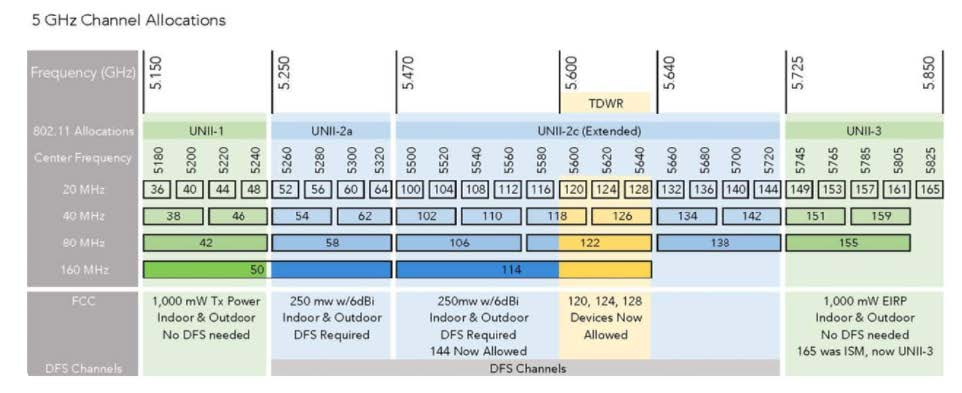
\includegraphics[width=\linewidth]{fotos_ema/canales_frec}
\caption{canales presentes en el rango de frecuencia de 5.725 a 5.825 MHz.}
\label{fig:canales_frec}
\end{figure}

 Al entrar más en detalle en las características de cada canal disponible, se usará el canal 155 que posee las características expuestas en la tabla \ref{tab:carac_155}. 
 Estos datos son sacados del Listado de canales WLAN\footnote{\href{https://en.m.wikipedia.org/wiki/List_of_WLAN_channels}{Listado de canales WLAN}}.

\begin{table}[htbp]
  \resizebox{\textwidth}{!}{%
  \centering
  \begin{tabular}{|c|p{0.25\linewidth}|p{0.25\linewidth}|p{0.25\linewidth}|} 
    \hline 
    Número del canal: & Frecuencia de portadora en MHz: & Rango de frecuencias en MHz: & Ancho de banda del canal en MHz: \\ 
    \hline 
    155 & 5775 & 5735-5815 & 80 \\ 
    \hline 
  \end{tabular}}
\caption{características del canal 155.}
\label{tab:carac_155}
\end{table}

\subsection{Determinación de los equipos para el radioenlace troncal}

Teniendo en cuenta una tasa de transferencia de 255 Mbps, obtenida previamente, y una distancia entre Leandro N. Além y Quines de 35 kilómetros, se consideran los siguientes equipos presentes en la tabla \ref{tab:equipo_tronc_wireless}.
En la misma, se observan las distintas características obtenidas de las hojas de datos de los transmisores y antenas consideradas para conformar la red troncal. 
La opción 1 está formada por el transmisor AirFiber 5X HD y la antena AF-5G34-S45, ambos de la marca Ubiquiti, mientras que la opción 2 está formada por el transmisor B5c de la marca Mimosa y la antena HG5158DP-32D de la marca L-Com.



\begin{table}[htbp]
  
  \centering
  
    \begin{tabular}{|c|c|c|}
\cline{2-3}    \multicolumn{1}{r|}{} & \textbf{Opción 1} & \textbf{Opción 2} \bigstrut\\
    \hline
    \textbf{Transmisor} & AirFiber 5X HD\tablefootnote{\href{https://dl.ubnt.com/datasheets/airfiber/airFiber_5XHD_DS.pdf}{Datasheet AirFiber 5X HD}} & Mimosa B5c \tablefootnote{\href{https://mimosa.co/uploads/datasheets/Mimosa-by-Airspan-B5c-Datasheet_DS-0008-09.pdf}{Datasheet Mimosa B5c}}\bigstrut\\
    \hline
    \textbf{Tasa de transferencia} & 272,64 Mbps & 260 Mbps \bigstrut\\
    \hline
    \textbf{Ancho del Canal} & 80 MHz & 2x80 MHz \bigstrut\\
    \hline
    \textbf{Modulación} & 64 QAM MIMO & 64 QAM MIMO\bigstrut\\
    \hline
    \textbf{Potencia de salida} & 24 dBm & 24 dBm \bigstrut\\
    \hline
    \textbf{Sensibilidad del receptor} & -65 dBm  & -65 dBm \bigstrut\\
    \hline
    \textbf{Frecuencia de operación} & 5735-5815 MHz & 5735-5815 MHz \bigstrut\\
    \hline
    \textbf{Tipo de duplexación} & TDD & FDD \bigstrut\\
    \hline
    \textbf{Distancia alcance máximo} & Hasta 100 km & - \bigstrut\\
    \hline
    \textbf{Antena compatible} & AF-5G34-S45 \tablefootnote{\href{https://dl.ubnt.com/datasheets/airfiber/airFiber_Antennas_DS.pdf}{Datasheet AF-5G34-S45}}& HG5158DP-32D \tablefootnote{\href{https://www.l-com.com/Images/Downloadables/Datasheets/ds_HG5158DP-32D.pdf}{Datasheet HG5158DP-32D}}\bigstrut\\
    \hline
    \textbf{Ganancia de la antena} & 34 dBi & 32 dBi \bigstrut\\
    \hline
    \end{tabular}%
  \caption{características de los equipos a utilizar}
  \label{tab:equipo_tronc_wireless}%
\end{table}%

La tasa de transferencia se elije de tal manera que se puedan tener más de 255 Mbps de transferencia en downstream, que fue la tasa de transferencia que se calculó en la ecuación \ref{eq:tasa_de_bits_total}. 
El ancho del canal se elije teniendo en cuenta el valor que permita la tasa de transferencia deseada, sin aumentar exageradamente la modulación. 
Es por ello que en ambos casos se trabaja con el canal de 80 Mhz.  

Comparando ambos transmisores, se tiene que la opción 1 posee mejores prestaciones, ya que permite usar un ancho de canal hasta 100 MHz, mientras que la opción 2 sólo hasta 80 MHz. Además la marca Ubiquiti, posee mayor presencia en el país, un mejor servicio post-venta y un ecosistema más integrado.
Además el transmisor de la opción 1 garantiza una distancia de alcance de hasta 100 kilómetros, mientras que la opción 2, no brinda información. 
Finalmente, la antena de la opción 1 presenta mayor ganancia. 

Por lo mencionado anteriormente, es que se decidió utilizar los siguientes equipos para poder realizar el enlace punto a punto:

\begin{itemize}
    \item  AirFiber 5X HD
    \item  AF-5G34-S45
    \item  Cable Ethernet FTP CAT 6 24 AWG
    \item  Fichas RJ45 blindadas
\end{itemize}

Debido a que el equipo es \textit{all outdoor}, será necesario un cable ethernet que vaya desde la central hasta la ubicación del equipo en las alturas. 
Para ello, se utilizará un cable ETHERNET FTP CAT 6 24AWG, el cual permitirá alimentar el transmisor, además de realizar la transmisión de datos.
Teniendo en cuenta la calidad del cable, se deberá aumentar la tensión de alimentación para contrarrestar las pérdidas causadas por la resistencia interna del cable. 
En este caso, este tipo de cable presenta una resistencia de 4,1 $\Omega$ por metro. 
Por otro lado, el equipo transmisor se conecta a la antena, la cual no viene directamente integrada, por lo tanto, típicamente existe una pérdida debido a los conectores de 0,5 dB. 

\subsection{Determinación y simulación de los distintos enlaces}

Se procede a realizar la simulación de 3 posibles enlaces entre las localidades de Quines y Leandro N. Alem. 
Se logró realizar un enlace directo de 34,48 kilómetros, y dos enlaces con un repetidor en medio que permite utilizar torres de menor altura, rodeando los puntos altos que se encuentran entre las dos localidades. 
Si bien no es necesario utilizar un repetidor, se plantea como una posible alternativa, en caso que por factores externos, tales como clima, regulaciones presentes en la zona, disconformidad de parte de los habitantes, no se pueda ensamblar una torre de semejante altura.
Por otro lado, cabe destacar que las distintas torres se encuentran emplazadas cerca de un tendido eléctrico, el cual permitiría poder conectarse a la red eléctrica. 
En la tabla \ref{tab:altura_antenas}, se muestran las coordenadas de las antenas, para permitir la fácil ubicación de las mismas en un mapa online, así como las distintas alturas en las que se ubican para su simulación. 

\begin{table}[htbp]
  \resizebox{\textwidth}{!}{%
  \centering
    \begin{tabular}{|c|c|c|c|c|}
    \hline
    Identificación & Características & Conexión Directa & Conexión alternativa 1 & Conexión alternativa 2 \\
    \hline
    \multirow{3}[6]{*}{Leandro N.Alem} & Latitud & -32,47757 & -32,490972 & -32,490972 \\
\cline{2-5}         & Longitud & -66,05044 & -66,0553 & -66,0553 \\
\cline{2-5}         & Altura & 100 metros & 7 metros & 7 metros \\
    \hline
    \multirow{3}[6]{*}{Repetidor} & Latitud & -    & -32,433154 & -32,371145 \\
\cline{2-5}         & Longitud & -    & -66,014348 & -66,066243 \\
\cline{2-5}         & Altura & -    & 60 metros & 80 metros \\
    \hline
    \multirow{3}[6]{*}{Quines} & Latitud & -32,23412 & -32,234242 & -32,234242 \\
\cline{2-5}         & Longitud & -65,82269 & -65;802569 & -65,802569 \\
\cline{2-5}         & Altura & 70 metros & 70 metros & 30 metros \\
    \hline
    \end{tabular}}%
    \caption{ubicación y altura de las antenas presentes en la simulación.}
    \label{tab:altura_antenas}%
\end{table}%

A continuación en la Fig. \ref{fig:enlaces_radiom}, se muestran los tres enlaces implementados en el programa \textit{Radio Mobile}. 
Para una mejor visualización, se procede a presentar los distintos tramos implementados en las figuras \ref{fig:con_directa}, \ref{fig:con_alt} y \ref{fig:con_alt2}.

Una vez emplazadas las antenas, se procede a simular las distintas conexiones, obteniendo así más detalles de los enlaces, así como las zonas de Fresnel, las pérdidas y la P.I.R.E. En las figuras \ref{fig:sim_directa}, \ref{fig:sim_alt} y \ref{fig:sim_alt2} se presentan los datos obtenidos para la conexión directa, el primer enlace alternativo y el segundo enlace alternativo, respectivamente. 


\begin{figure}[htbp]
  \centering
  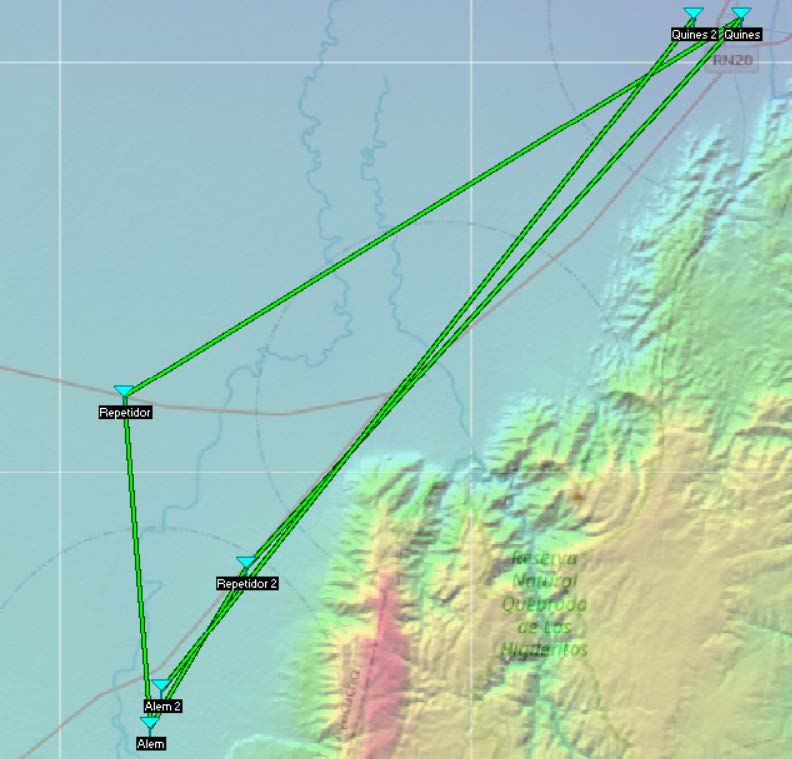
\includegraphics[width=\linewidth]{fotos_ema/imp_radio_mobile.jpg}
  \caption{implementación en Radio Mobile de los 3 enlaces.}
  \label{fig:enlaces_radiom}
\end{figure}
\clearpage
\subsubsection{Conexión directa}

En la Fig. \ref{fig:con_directa}, se presenta la conexión directa entre Leandro N. Alem y Quines.
La ventaja que presenta esta solución radica en el hecho de que se utilizan sólo dos transmisores, y 2 torres. El problema principal está en el hecho de que debido a la topografía del lugar, la altura necesaria para establecer la comunicación es mayor a las demás opciones, tal como se muestra en la tabla \ref{tab:altura_antenas}.

\begin{figure}[htbp]
  \centering
  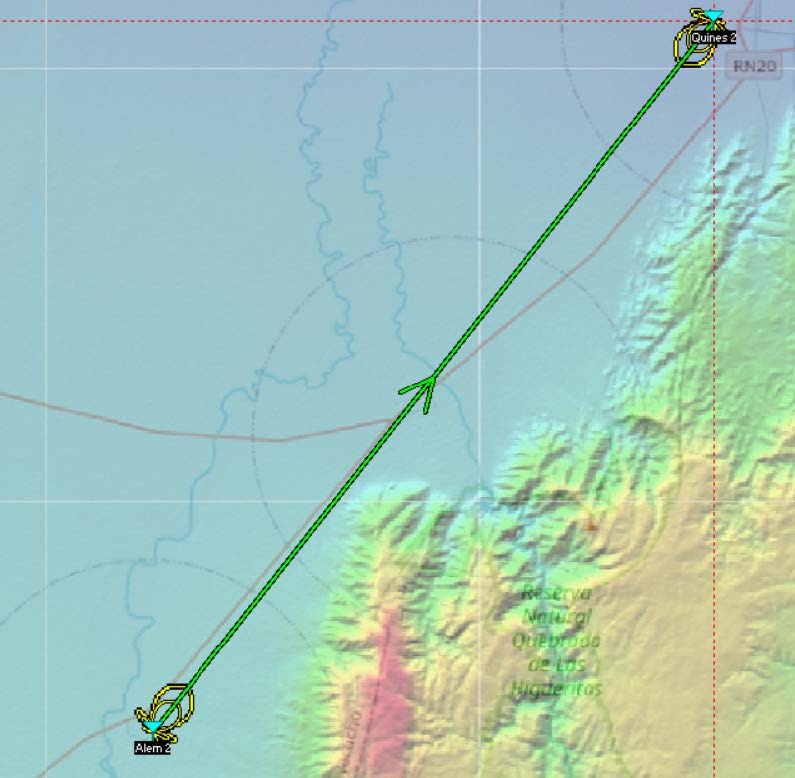
\includegraphics[width=0.55\linewidth]{fotos_ema/con_directa.jpg}
  \caption{conexión directa entre Leandro N. Alem y Quines.}
  \label{fig:con_directa}
\end{figure}
En la Fig. \ref{fig:sim_directa} se muestra el resultado de la simulación, demostrando con la misma el teorico funcionamiento del mismo.
\begin{figure}[htbp]
  \centering
  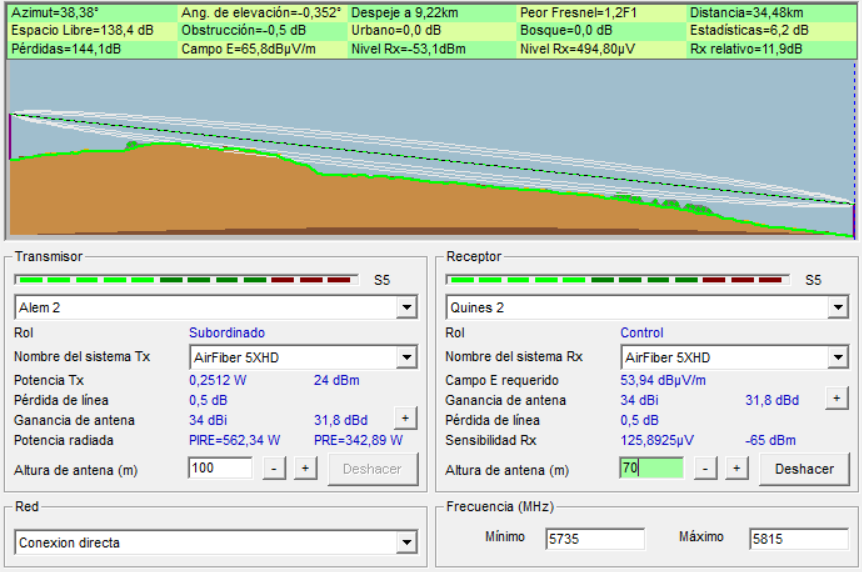
\includegraphics[width=0.7\linewidth]{fotos_ema/sim_directa.png}
  \caption{simulación de la conexión directa entre Leandro N. Alem y Quines.}
  \label{fig:sim_directa}
\end{figure}

\subsubsection{Primera conexión alternativa con repetidor}
En la Fig. \ref{fig:con_alt} se presenta el tramo entre Leandro N. Alem y el repetidor de la primera conexión alternativa, y la conexión entre ese repetidor y Quines.

\begin{figure}[ht!]
  \centering
  \subcaptionbox{conexión alternativa entre Leandro N. Alem y el repetidor.}%
  [.48\linewidth]{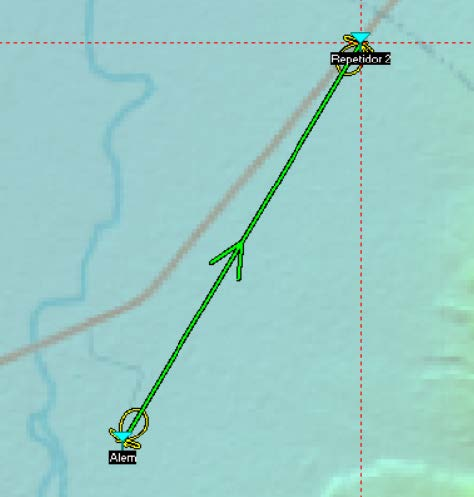
\includegraphics[height=11\baselineskip]{fotos_ema/con_alt_alem_rep.jpg}}%
  \subcaptionbox{conexión alternativa entre el repetidor y Quines.}
  [.48\linewidth]{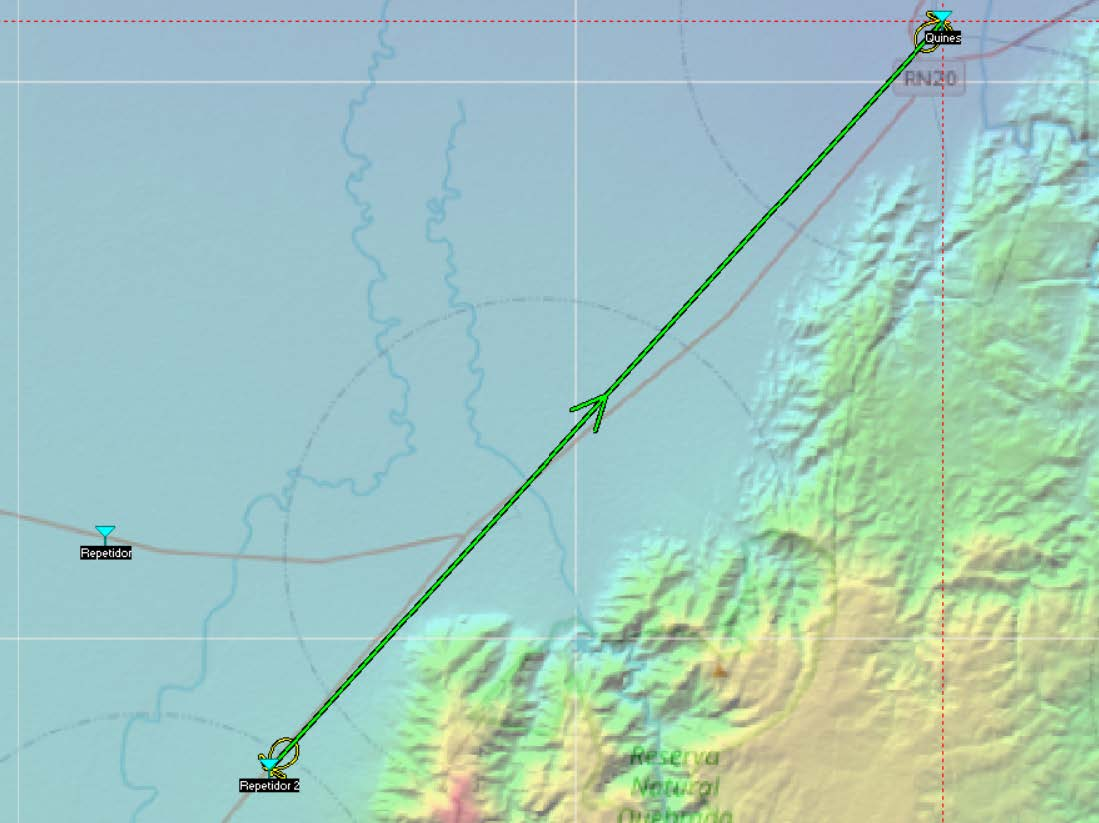
\includegraphics[height=11\baselineskip]{fotos_ema/con_alt_rep_quines.jpg}}
  \caption{conexión alternativa entre Leandro N. Alem y Quines.}
  \label{fig:con_alt}
\end{figure}

En la Fig. \ref{fig:sim_alt} se presenta la simulación obtenida para el tramo entre Leandro N. Alem y el repetidor de la primera conexión alternativa, y la simulación de la conexión entre ese repetidor y Quines.
Gracias a dicha simulación se comprueba el funcionamiento teorico del enlace.
Esta alternativa presenta la ventaja de que las alturas necesarias para las antenas no son tan altas como para la conexión directa.
Sin embargo, es necesario usar más torres y equipos de transmisión lo cual no solo presenta mayores costos, sino también mayores problemas a la hora de tramitar permisos y mantener la instalación.

\begin{figure}[ht!]
  \centering
  \subcaptionbox{simulación de la conexión alternativa entre Leandro N. Alem y el repetidor.}%
  [.48\linewidth]{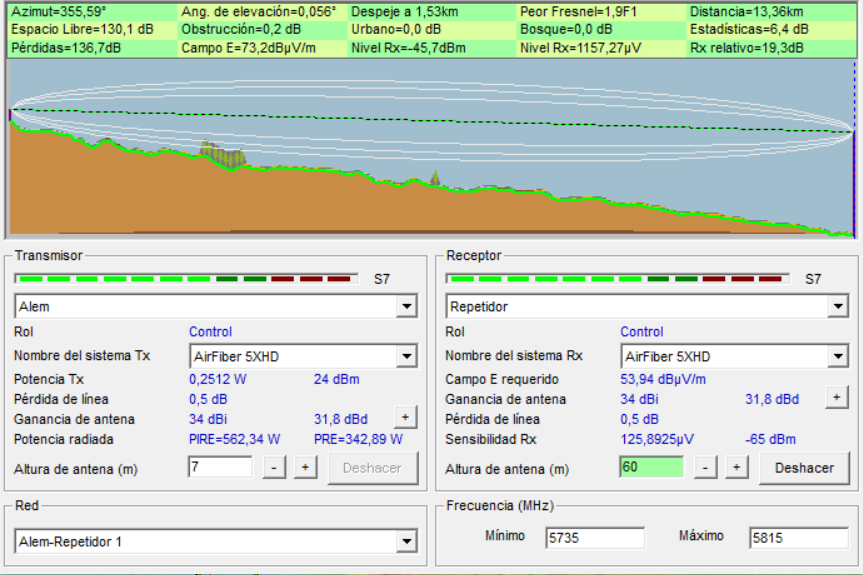
\includegraphics[height=10\baselineskip]{fotos_ema/sim_alt_alem_rep}}%
  \hfill%
  \subcaptionbox{simulación de la conexión alternativa entre el repetidor y Quines.}
  [.48\linewidth]{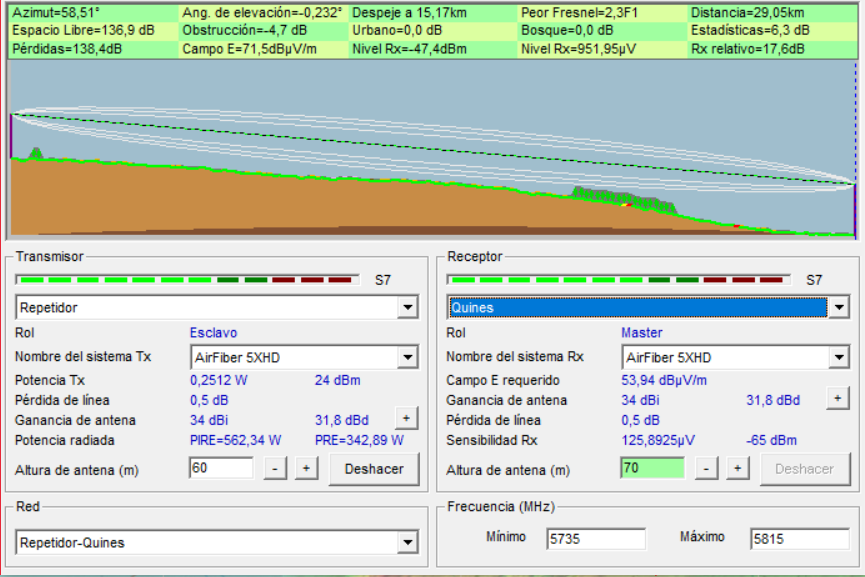
\includegraphics[height=10\baselineskip]{fotos_ema/sim_alt_rep_quines}}
  \caption{simulación de la conexión alternativa entre Leandro N. Alem y Quines.}
  \label{fig:sim_alt}
\end{figure}

\clearpage

\subsubsection{Segunda conexión alternativa con repetidor}

A continuación, se presenta en la Fig. \ref{fig:con_alt2}, la conexión entre la localidad de Leandro N. Alem y el repetidor de la segunda conexión alternativa, y la conexión entre dicho repetidor y Quines.


\begin{figure}[ht!]
  \centering
  \subcaptionbox{segunda conexión alternativa entre Leandro N. Alem y el repetidor.}%
  [.48\linewidth]{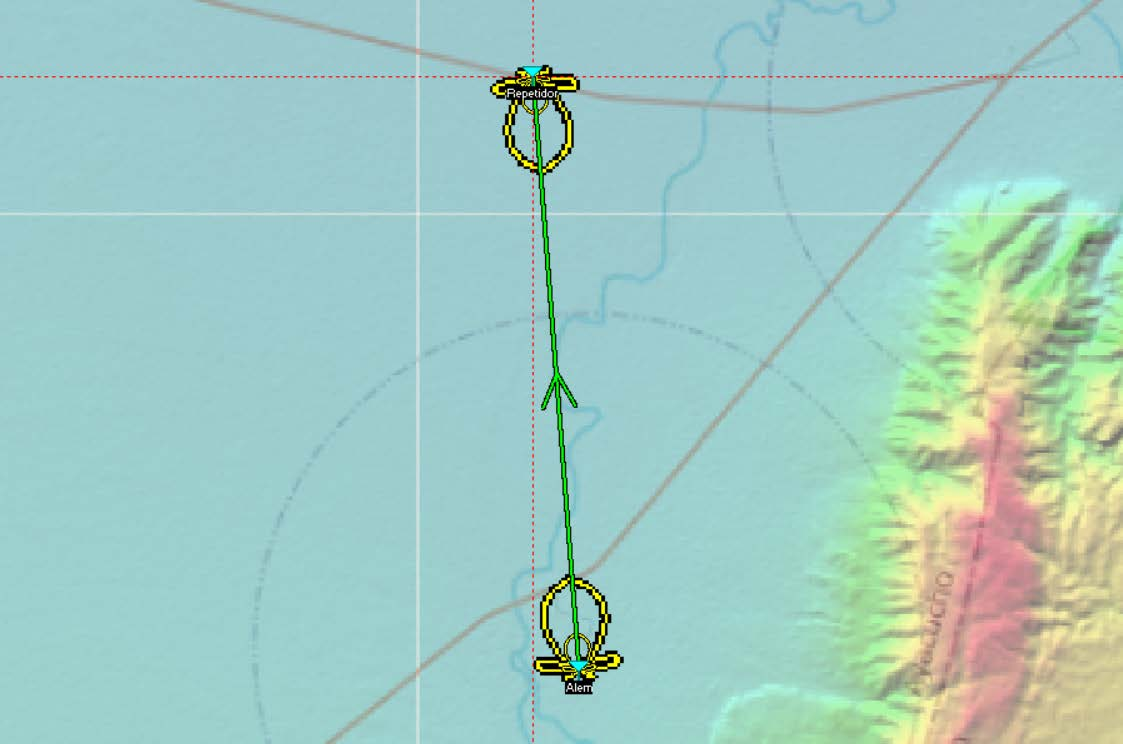
\includegraphics[height=8.5\baselineskip]{fotos_ema/con_alt2_alem_rep.jpg}}%
  \hfill%
  \subcaptionbox{segunda conexión alternativa entre el repetidor y Quines.}
  [.48\linewidth]{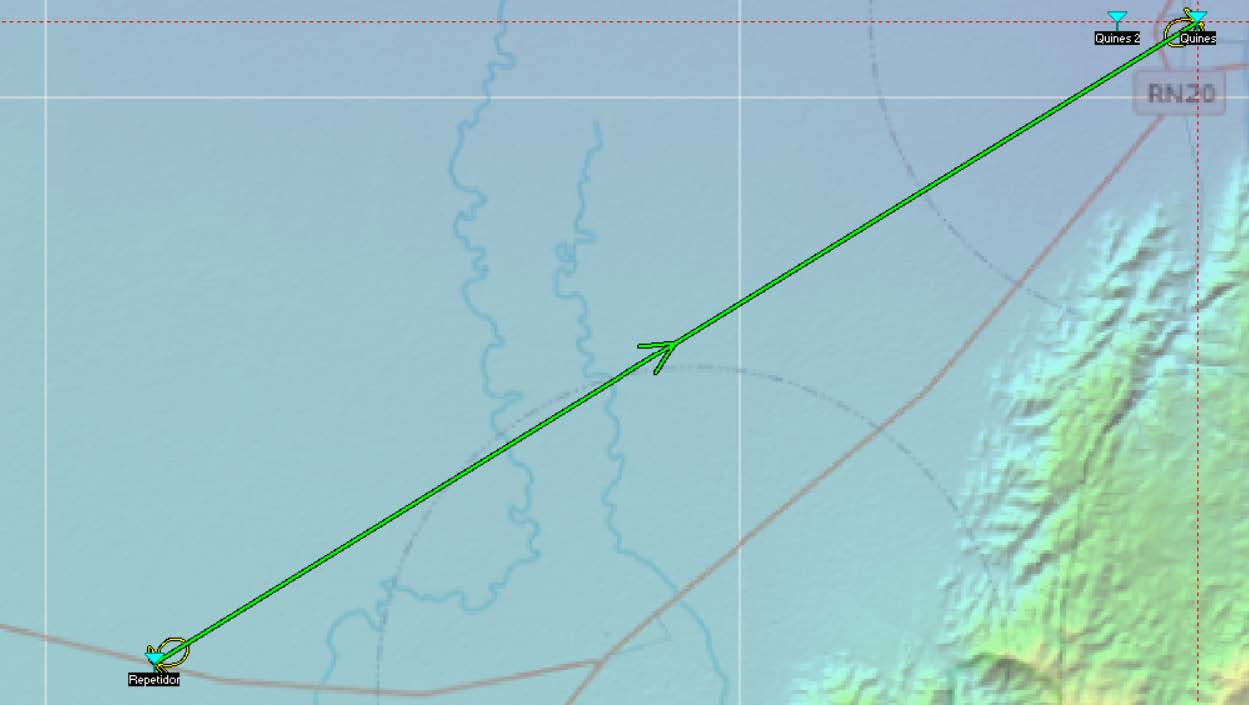
\includegraphics[height=8.5\baselineskip]{fotos_ema/con_alt2_rep_quines.jpg}}
  \caption{segunda conexión alternativa entre Leandro N. Alem y Quines.}
  \label{fig:con_alt2}
\end{figure}

En la Fig. \ref{fig:sim_alt2} se presenta la simulación obtenida para el tramo entre Leandro N. Alem y el repetidor de la primera conexión alternativa, y la simulación de la conexión entre ese repetidor y Quines.
Gracias a dicha simulación se comprueba el funcionamiento teorico del enlace.
Al igual que la anterior, esta alternativa presenta la ventaja de que las alturas necesarias para las antenas no son tan altas como para la conexión directa, pero también es necesario usar más torres y equipos de transmisión. 
La diferencia con la opción anterior radica en una menor altura en total, sumando las alturas de todas las antenas.

\begin{figure}[ht!]
  \centering
  \subcaptionbox{simulación de la segunda conexión alternativa entre Leandro N. Alem y el repetidor.}%
  [.48\linewidth]{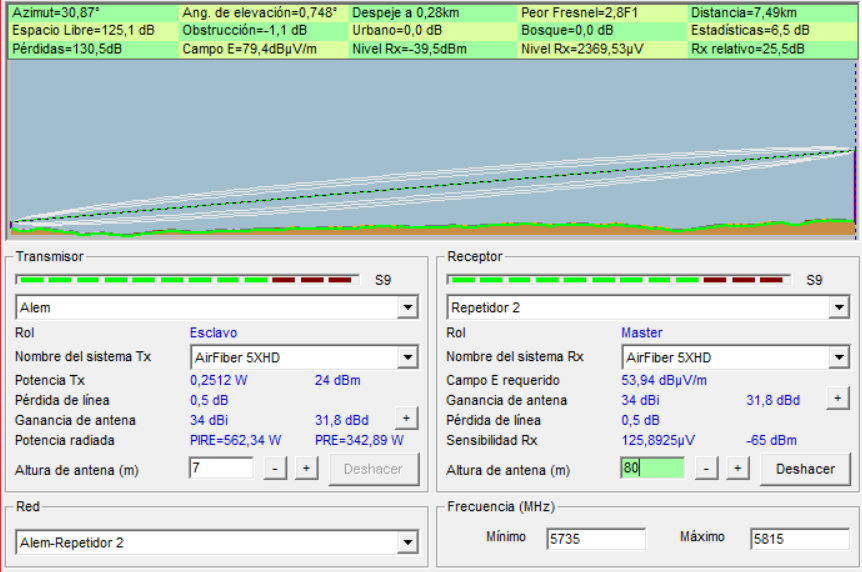
\includegraphics[height=10\baselineskip]{fotos_ema/sim_alt2_alem_rep}}%
  \hfill%
  \subcaptionbox{simulación de la segunda conexión alternativa entre el repetidor y Quines.}
  [.48\linewidth]{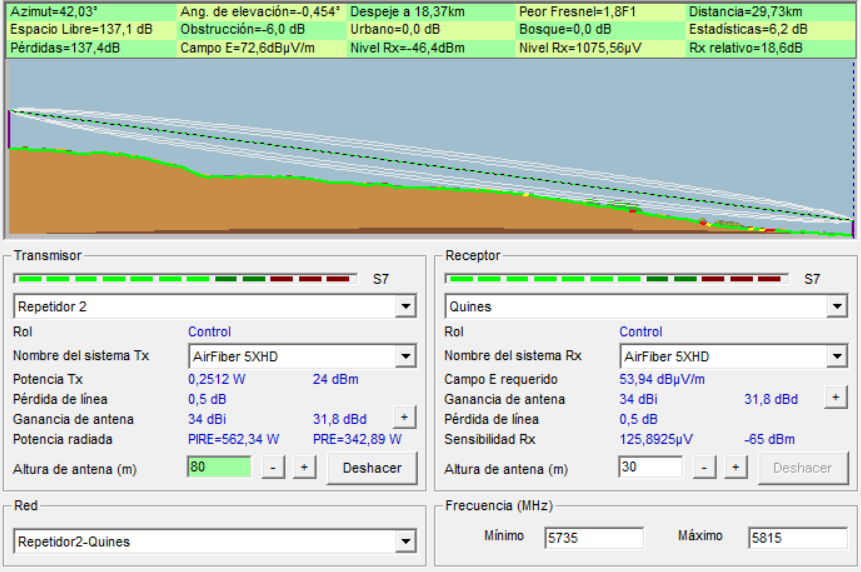
\includegraphics[height=10\baselineskip]{fotos_ema/sim_alt2_rep_quines}}
  \caption{simulación de la segunda conexión alternativa entre Leandro N. Alem y Quines.}
  \label{fig:sim_alt2}
\end{figure}

\clearpage
\subsubsection{Elección del tipo de enlace}
Observando los distintos enlaces propuestos, se decide optar por la conexión directa, ya que la misma presenta las siguientes ventajas:

\begin{itemize}
  \item  \textbf{Emplazamiento de 2 torres:} esta configuración necesita para su operación el emplazamiento de solamente 2 torres. 
  Si bien las opciones con repetidor necesitan torres de menor altura para su operación, el hecho de tener que armar una torre adicional, junto con 2 equipos, los cuales necesitan además supervisión técnica y mantenimiento, encarece en tal manera el sistema, que se justifica la utilización de solamente dos torres. 
  Aún más, el hecho de instalar una torre adicional, aunque sea de menor altura, deviene en mayores gastos administrativos, legales y técnicos, convirtiendo así a la conexión directa en la opción más asequible y sencilla.

  \item \textbf{ Menor mantenimiento:} debido a que solo se cuenta con 2 equipos, en lugar de 4, como lo es en el caso de las conexiones con repetidor, el mantenimiento de la instalación necesaria es menor.

  \item \textbf{ Mejor aprovechamiento del equipo a utilizar:} debido a los requerimientos de potencia y tasa de transferencia de bits, era necesario utilizar un equipo con las prestaciones previamente mencionadas, sin embargo, el equipo soporta conexiones de hasta 100 kilómetros de distancia. 
  Al colocar un repetidor en un radio cercano al emisor, se está desaprovechando esta capacidad, sobredimensionando el sistema, debido a que no existe un equipo que cubra menores distancias pero que cuente con las tasas de transferencia de bits necesarias.
\end{itemize}

\subsection{Cálculos analíticos}

\subsubsection{Ganancia del sistema}

Teniendo en cuenta los elementos en el sistema que contribuyen positivamente a aumentar la potencia de la señal podemos considerar a estos como ganancias en el sistema. Entre estos elementos consideramos a:

\begin{itemize}
  \item  La potencia de Tx ($P_{TX}$[dBm]) que corresponde a la potencia de RF que puede entregar el equipo. En este caso la potencia del transmisor AirFiber 5X HD es de 24 dBm como muestra la tabla \ref{tab:equipo_tronc_wireless}. 

  \item  La ganancia de la antena  ($G_{TX}$[dB])  utilizada es de 34 dBi mostrada en la tabla \ref{tab:equipo_tronc_wireless}.  
  La antena junto con el transmisor anteriormente mencionado se encuentra ubicado en en la localidad de Quines con LOS hacia la antena receptora ubicada en Leandro N. Alem. 

  \item  La sensibilidad de Rx ($S_{RX}$[dBm]) que indica cuanta potencia necesita el receptor para poder interpretar los datos recibidos es de -65 dBm como muestra la tabla \ref{tab:equipo_tronc_wireless}.
\end{itemize}

\subsubsection{Pérdidas del sistema}

A continuación se tienen en cuenta los elementos en el sistema que contribuyen negativamente en el sistema y son tomados como pérdidas para el mismo: 

\begin{itemize}
  \item  Los conectores (${At}_1$[dB]) que son empleados para inyectar la señal RF en el cable hacia la antena se presentan como una pérdida para el sistema de aproximadamente 0,5 dB.

  \item  Los cables (${At}_2$[dB]) que son empleados para llevar la señal de RF a la antena también presentan pérdidas de potencia en la señal y esta depende del tipo de cable. Dado que el equipo utilizado es de tipo all outdoor, las pérdidas son despreciables.

  \item  Las atenuaciones en el espacio libre ($L_b$[dB]) expresada como:
  \begin{equation}
    L_b=20\log{D} [\text{ km}]+20\log{f} [\text{ GHz}]+92,45
    \label{eq:at_free_sp}
  \end{equation}
  Donde $D$ es la distancia entre antenas y $\ f$ es la frecuencia de portadora. 

  La distancia entre la antena transmisora y la antena receptora es $D=34,48$ km y $f=5,775$ GHz, reemplazando en la ecuación \ref{eq:at_free_sp}, la atenuación por espacio libre da como resultado:
  \begin{equation*}
    L_b=20\log{34,48}+20\log{5,775}+92,45=138.43 \text{ dB} 
  \end{equation*}
  

\end{itemize}


\subsubsection{Presupuesto de potencia completo}
  
Para realizar el presupuesto de enlace se utilizó la ecuación de FRIIS:

\begin{equation}
  P_{TX}[\text{dBm}]-S_{RX}[\text{dBm}] \geq \Sigma \text{ Pérdidas} -\Sigma\text{ Ganancias} + \text{FM}
  \label{eq:friis} 
\end{equation}



Donde la sumatoria de las pérdidas involucra a las pérdidas por conectores, por cables y por el espacio libre  mencionadas anteriormente. 
Por otro lado la sumatoria de las ganancias corresponde a las ganancias de las antenas y FM es el margen de desvanecimiento que permite considerar las características no ideales y menos predecibles de la propagación de las ondas radioeléctricas en el espacio libre, como las pérdidas por trayectos múltiples y la sensibilidad del terreno.

Para calcular el margen de desvanecimiento FM se utiliza la ecuación de Barnett-Vignant.
\begin{equation}
  \text{FM}=30\log{D}[\text{km}]+10\log{(6ABf)}[\text{GHz}]-10\log{(1-R)}-70
  \label{eq:vignant}
\end{equation}

Donde :

\begin{itemize}
\item   R es la Confiabilidad y se expresa en decimales (de 0 a 1); típica: 0,995
\item  (1-R) es el objetivo de confiabilidad para una trayectoria de 400 km en un solo sentido o dirección
\item   A es el factor de rugosidad: A = 1 sobre terreno normal promedio.
\item   B es el factor para convertir una probabilidad del peor mes a una probabilidad anual: B = 1 para una disponibilidad anual a una base para el peor mes.
\end{itemize}

Reemplazando en la ecuación \ref{eq:vignant} se obtiene: 

\begin{eqnarray}
  \text{FM}&=&30\log{34,48}[\text{km}]+10\log{(6*1*1*5,775)}[\text{GHz}]-10\log{(1-0.995)}-70 \nonumber\\
  \text{FM}&=&14.53\text{ dB}
  \label{eq:res_vignant}
\end{eqnarray}


Finalmente, reemplazando los resultados obtenidos de la ecuación \ref{eq:at_free_sp} y ecuación \ref{eq:res_vignant} en la ecuación \ref{eq:friis}: 

\begin{eqnarray*}
  G_S[\text{dB}]&=&P_{TX}[\text{dBm}]-S_{RX}[\text{dBm}] \geq (L_{TT}+L_b+L_{TR}) -(G_{TX}+G_{RX})+FM \\ 
G_S[\text{dB}]&=&24-(-65) \geq  (138.43+0,5)-(34+34)+14,53 \\ 
G_S[\text{dB}]&=&89 \geq 85.03 
\end{eqnarray*}

Comparando las ganancias y las pérdidas, se puede concluir que el enlace es viable. 
Hay una diferencia de 3,97 dB como margen adicional frente a otras posibles interferencias. 
Sumando esta diferencia con el margen de desvanecimiento FM podemos obtener un valor de Rx relativo igual a 18,5 dB. 
El Rx relativo se diferencia en 6,6 dB del calculado por el software Radio Mobile, siendo este de 11,9 dB como muestra la Fig. \ref{fig:sim_directa}. 
Esto se debe a que el software tiene en cuenta otros parámetros que no aparecen en la ecuación de FRIIS, como pérdidas por bosque y otro tipo de obstrucciones.

\section{Red de acceso con radioenlace}

\subsection{Determinación de la tasa de transferencia necesaria y cálculo de los accesos}

Del estudio socioeconómico realizado sobre la localidad de Leandro N. Alem se obtuvo que 83 hogares del total de la población serán potenciales clientes del servicio brindado. 
También se obtuvo como conclusión que 25 clientes optarán por el pack básico, 44 clientes utilizarán el pack intermedio y 14 clientes el pack premium. 
En la Tabla~1 se observa un resumen de los valores más importantes a tener en cuenta.


\begin{table}[htbp]
  \resizebox*{\textwidth}{!}{
  \centering
  \begin{tabular}{|c|p{0.2\linewidth}|p{0.2\linewidth}|p{0.2\linewidth}|p{0.2\linewidth}|} 
  \hline 
  \textbf{Servicio} & \textbf{Tasa de datos} & \textbf{Pack básico} & \textbf{Pack intermedio} & \textbf{Pack premium} \\ \hline 
\textbf{Canal SDTV} & 1.5 Mbps & 50 canales & 50 canales & 50 canales \\ \hline 
\textbf{Canal HDTV} & 6 Mbps & - & - & 6 canales \\ \hline 
\textbf{VoIP\footnote{ La tasa de datos es despreciable a la hora de realizar los cálculos.}} & 30 kbps & 30 kbps & 30 kbps & 30 kbps \\ \hline 
\textbf{Internet} & - & - & 6 Mbps & 15 Mbps \\ \hline 
\textbf{Clientes} & - & 25 & 44 & 14 \\ \hline 
\end{tabular}}%
\caption{contenido de pack de servicios.}
\label{tab:cont_pack_servicio}
\end{table}
 



 Según el Ministerio de Planificación Federal, Inversión Pública y Servicios, en el año 2.009, en la República Argentina había aproximadamente 10 millones de hogares y cerca de 12 millones de televisores\footnote{\href{http://www.infoleg.gob.ar/basehome/actos_gobierno/actosdegobierno14-9-2009-2.htm}{Televisores por hogar}}. 
 Se estima entonces que la cantidad de televisores supera en un 20\% la cantidad de hogares. 
 Este porcentaje no se distribuye uniformemente sobre la población, varía según el poder adquisitivo de las personas y por consiguiente lo hace sobre los clientes, siendo más frecuente que una persona con un buen sueldo tenga más de un televisor. 
 Por lo tanto, se puede decir que el 20\% de los 83 potenciales clientes, que corresponde a 17 clientes, tienen 2 televisores.
Si se considera un máximo de 2 televisores por hogar y el poder adquisitivo de cada grupo, se estima que 8 clientes correspondientes al pack premium cuentan con dos televisores, 6 clientes en el pack intermedio y 3 en el pack básico.
El resto de los clientes solo cuentan con un televisor. 
Además, se considera que los clientes pertenecientes a los pack intermedios y premium hacen uso del 60\% de los megas correspondientes a cada pack.

La tasa de transferencia en el peor de los casos para el pack premium da como resultado 18,42 Mbps, como muestra la ecuación \ref{eq:tasa_transf_premium}. 
Esto se calcula de suponer que 8 clientes de los 14 (57\%) usan 2 canales HD simultáneamente, 6 clientes (43\%) utilizan solo un canal HD, sumando además el un factor de simultaneidad del 60\% en el internet. 


\begin{equation}
  2*6x{10}^6*0.57+6x{10}^6*0.43+0.6*15x{10}^6=18.42 \text{ Mbps}
  \label{eq:tasa_transf_premium}
\end{equation}


De forma similar se realizaron los cálculos para los pack intermedios y básicos. 
Los resultados se muestran en la ecuación \ref{eq:tasa_transf_int} y ecuación \ref{eq:tasa_transf_basic} respectivamente. 


\begin{equation}
 2*1.5x{10}^6*0.136+1.5x{10}^6*0.863+ 0.6*6x{10}^6=5,3 \text{Mbps} 
 \label{eq:tasa_transf_int}
\end{equation}

\begin{equation}
 2*1.5x{10}^6*0.12+1.5x{10}^6*0.88=1,68 \text{ Mbps}
 \label{eq:tasa_transf_basic}
\end{equation}
 

 En la Fig. \ref{fig:cuadrantes_alem} se puede observar en rojo los cuadrantes en los cuales se concentra mayor cantidad de gente y con un icono verde la ubicación de las antenas de la Autopista de la Información. 
 Observando el tamaño de los hogares, se supone que los grupos con mayor poder adquisitivo se encuentran entre los cuadrantes que van del 1 al 6, los cuales pueden ser potenciales clientes de los packs intermedio y premium. 
 Sin embargo, entre los cuadrantes 1 y 2 se encuentra una antena Wi-Fi (5 GHz) brindando internet gratis por parte del gobierno. 
 Considerando esto se decidió tener prioridad en los cuadrantes 3, 4, 5 y 6 a la hora de decidir la ubicación del Access Point (AP). Por otra parte, los cuadrantes del 11 al 14 no se ven alcanzados por ninguna antenas del gobierno, por lo que se estima que brindando un servicio que antes no disponían se encontrarán potenciales clientes en esta zona. 
 Por último está la zona céntrica donde se encuentra la plaza, en los cuadrantes 9 y 10. Esta zona cuenta con una antena Wi-Fi (2,4 GHz) pero la misma se encuentra saturada, rondando en promedio los 45 clientes\footnote{\href{http://wifi.sanluis.gov.ar/}{Antenas Wi-Fi de la provincia de San Luis}}.


\begin{figure}[htbp]
  \centering
  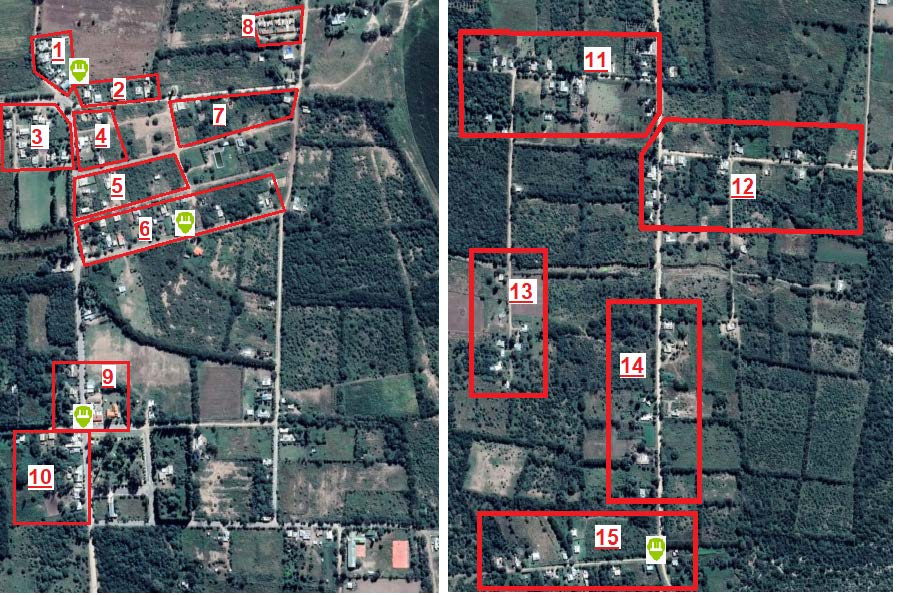
\includegraphics[width=0.75\linewidth]{fotos_ema/cuadrantes_alem.jpg}
  \caption{a la izquierda la zona norte y a la derecha la zona sur de la localidad de leandro N. Alem.}
  \label{fig:cuadrantes_alem}
\end{figure}

La cantidad de AP que se utilizarán para lograr la mayor cobertura posible y brindarle el servicio a los clientes se calcula a partir de la tasa de transferencia requerida por cliente teniendo en cuenta el peor de los casos.
Para el siguiente cálculo se optó por no considerar el pack básico, de esta forma se sobredimensiona el sistema para un futuro crecimiento en caso de que nuevos clientes quieran adquirir el servicio y/o aquellos que quieran adquirir un mejor pack. 
El promedio entre el caso más desfavorable de los pack intermedio y premium da como resultado 11,86 Mbps como se observa en la ecuación \ref{eq:prom_desf}. 

\begin{equation}
  \frac{18.426x{10}^6+5.3x{10}^6}{2}=11.86 \text{ Mbps}
  \label{eq:prom_desf}
\end{equation}

La tasa de transferencia total para brindar el servicio viene dada por el valor de la Ecuación \ref{eq:prom_desf} multiplicada por cantidad de clientes. Esto se ve reflejado en la ecuación \ref{eq:total_mbps_need}:

\begin{equation}
  83 * 11.86x{10}^6 = 984.38 \text{ Mbps}
  \label{eq:total_mbps_need}
\end{equation}

de los cuales se estima que por la cantidad de casas que se observan en la figura \ref{fig:cuadrantes_alem}, el 80 \% de la población vive en los cuadrantes del 1 al 9 y el 20\% restante se encuentra distribuido entre los cuadrantes 10 al 15. 
Teniendo en cuenta esta distribución de la población, se utilizarán AP que trabajen en la banda de 2,4 GHz y 5 GHz, de esta forma los clientes que se encuentran distribuidos en los extremos de la localidad serán alcanzados por las antenas de 2,4 GHz ya que estas cuentan con mayor alcance a costas de menor transferencia de bits. 
Por otro lado, en las partes que concentran mayor cantidad de clientes se utilizarán AP que trabajen en 5 GHz brindando una mayor tasa de transferencia pero menor alcance.

Hay que considerar que las antenas elegidas deben tener una tasa bruta de el doble de la tasa de transferencia calculada en la ecuación \ref{eq:total_mbps_need} ya que se pierde alrededor del 50\% de la capacidad de transmisión para garantizar que  la información se transmite de forma segura. 
Siendo así, la tasa de transferencia total es de 1.968 Mbps. 
Sin embargo, esta tasa de transferencia se distribuye entre los equipos cuando la cantidad de APs utilizadas aumenta y no es necesario que un solo equipo soporte el total. 

\subsection{Elección de los puntos de acceso}

La elección de los AP se basó en la tasa de transferencia necesaria calculada en el punto anterior. 
A continuación se mostrarán las características de los dos equipos AP que se analizaron: Aruba AP-375 y Altai A3-Ei.

En la tabla \ref{tab:carac_aruba_AP375} se observa la potencia del transmisor y la sensibilidad de recepción del equipo Aruba AP-375, además de su familia de protocolos, tipo de antena y tasa de transferencia\footnote{\href{https://www.arubanetworks.com/assets/ds/DS_AP370Series.pdf}{Datasheet Aruba AP-375}}. 
Tanto la potencia del transmisor, como la sensibilidad del receptor, poseen un rango de valores que varía dependiendo el tipo de modulación elegida.

\subsubsection{Características Aruba AP-375}

\begin{table}[htbp]
  \resizebox*{\textwidth}{!}{
\centering
\begin{tabular}{|p{0.1\textwidth}|p{0.2\textwidth}|p{0.2\textwidth}|p{0.2\textwidth}|p{
0.2\textwidth}|p{0.1\textwidth}|} 
\hline 
\textbf{Banda de frecuencia} & \textbf{Tasa de transmisión} & \textbf{Antena} & \textbf{Rango potencia transmisor} & \textbf{Rango sensibilidad receptor} & \textbf{Familia protocolos} \\ 
\hline 
2,4 GHz & Hasta 300 Mb/s & 2x2 MIMO\newline omnidireccional  & Max: 23 dBm\newline Min: 18 dBm & Min: -93 dBm\newline Max: -71 dBm & 802.11n \\ 
\hline 
5 GHz & 1733 Mb/s & 4x4 MU-MIMO\newline omnidireccional & Max: 22 dBm\newline Min: 15 dBm & Min: -87 dBm\newline Max: -61 dBm & 802.11ac \\ 
\hline 
\end{tabular}}
\caption{características de AP Aruba AP-375.}
\label{tab:carac_aruba_AP375}
\end{table}

Al analizar el equipo en la frecuencia de 2,4 GHz por medio de su datasheet se puede observar en la tabla \ref{tab:anchos_banda_canal} que dependiendo el tipo de modulación MCS a usar, también se tienen diferentes anchos de banda del canal. 
En el modo HT20 es de 20 MHz, y en el modo HT40 es de 40 MHz. 

\begin{table}[htbp]
  \centering
    \begin{tabular}{|c|c|c|}
    \hline
    \multicolumn{3}{|c|}{802.11n(2,4 GHz): 6,5 to 300 (MCS0 to MCS15)} \bigstrut\\
    \hline
    \multicolumn{3}{|l|}{802.11n HT20 2,4 GHz} \bigstrut\\
    \hline
    MCS0/8 & 25   & -93 \bigstrut\\
    \hline
    MCS7/15 & 18   & -71 \bigstrut\\
    \hline
    \multicolumn{3}{|l|}{802.11n HT40 2,4 GHz} \bigstrut\\
    \hline
    MCS0/8 & 22   & -90 \bigstrut\\
    \hline
    MCS7/15 & 18   & -68 \bigstrut\\
    \hline
    \end{tabular}%
  \caption{anchos de banda de canal.}
  \label{tab:anchos_banda_canal}%
\end{table}%
 

Como la tasa de transferencia del equipo es de hasta 300 Mbps, se busca este valor en la tabla MCS Index\footnote{\href{https://wlanprofessionals.com/mcs-table-and-how-to-use-it/}{Tabla MCS y como usarla}} y se obtienen los valores mostrados en las Fig. \ref{fig:msc_index_2_4GHz}. 
Una tabla MCS es una búsqueda que se puede utilizar para encontrar qué velocidad de datos se negociará entre dos estaciones una vez que se conocen todos los parámetros de conexión. 
Para cada combinación posible de modulación, tasa de codificación, número de flujos espaciales, ancho de canal e intervalo de guarda, existe un índice MCS único.


\begin{figure}[htbp]
  \centering
  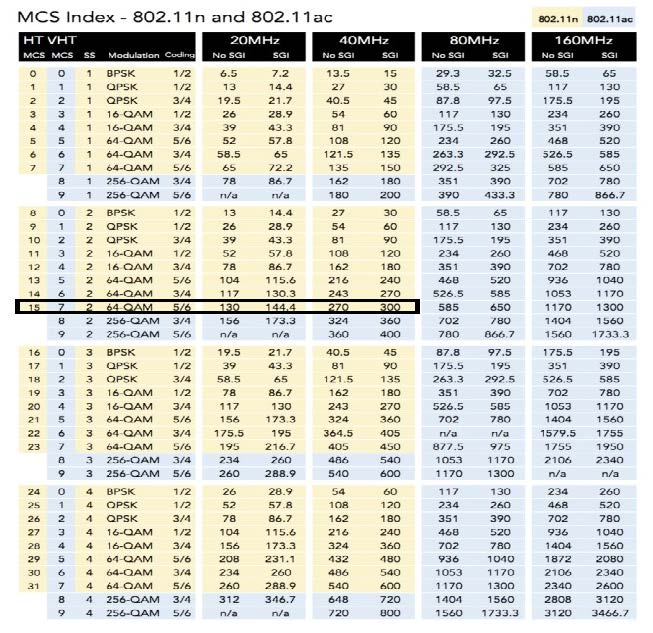
\includegraphics[width=0.5\linewidth]{fotos_ema/msc_index_2_4GHz.jpg}
  \caption{MSC Index-Análisis para 2,4 GHz.}
  \label{fig:msc_index_2_4GHz}
\end{figure}


Finalmente, se opta por usar el ancho de banda en el modo HT40 ya que con este se obtiene la tasa de transferencia máxima para una frecuencia de 2,4 GHz.

Para realizar el análisis en la frecuencia de 5 GHz, se deben tener en cuenta el ancho de banda de canal, cantidad de flujos espaciales (SS) y el tipo de modulación. 
Por medio del datasheet del equipo, se obtiene la Fig. \ref{fig:msc_index_2_4GHz} que indica que para una modulación MCS entre 0 y 9, con un flujo espacial entre 1 y 4 y con un ancho de banda de canal entre 20,40 y 80 MHz, se obtiene una tasa de transferencia de hasta 1733 MBps.

\begin{figure}[htbp]
  \centering
  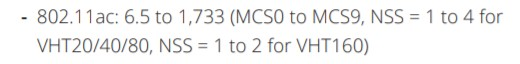
\includegraphics[width=0.5\linewidth]{fotos_ema/carac_ap_1733.jpg}
  \caption{Características de AP para una tasa de transferencia de 1733 Mbps.}
  \label{fig:carac_ap_1733}
\end{figure}

Luego, se recurre al MCS Index para encontrar la modulación requerida. 
Esto se muestra en la Fig. \ref{fig:msc_index_5_GHz}.

\begin{figure}[htbp]
  \centering
  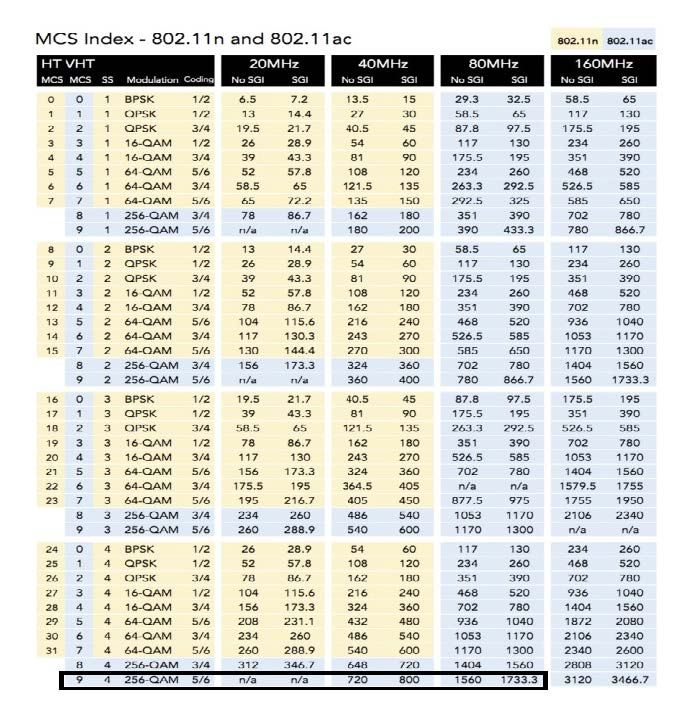
\includegraphics[width=0.5\linewidth]{fotos_ema/msc_index_5_GHz.jpg}
  \caption{Características de AP para una tasa de transferencia de 1733 Mbps.}
  \label{fig:msc_index_5_GHz}
\end{figure}


\subsubsection{Características Altai A3-Ei}

De igual manera, se analiza el AP Altai A3-Ei, mostrando los datos de la datasheet\footnote{\href{https://www.altaitechnologies.com/portfolio-item/a3-ei/}{Datasheet Altai A3-Ei}} en la tabla \ref{tab:carac_AP_altai}.

\begin{table}[htbp]
  \resizebox*{\textwidth}{!}{
  \centering
    \begin{tabular}{|c|c|c|p{0.2\textwidth}|p{0.2\textwidth}|c|} 
    \hline 
    \textbf{Banda de frecuencia} & \textbf{Tasa de transmisión} & \textbf{Antena} & \textbf{Rango potencia transmisor} & \textbf{Rango sensibilidad receptor} & \textbf{Familia protocolos} \\ 
    \hline 
    2,4 GHz & Hasta 450 MBps & 3x3:3 MIMO & Max:30 dBm \newline Min: 25 dBm & HT20: -92dBm \newline HT40: -88dBm & 802.11n \\ 
    \hline 
    5 GHz & Hasta 1300 MBps & 3x3:3 MIMO & Max:30 dBm \newline Min: 25 dBm & HT20: -92dBm \newline HT40: -88dBm & 802.11ac \\ 
    \hline 
\end{tabular}}
\caption{características AP Altai A3-Ei.}
\label{tab:carac_AP_altai}
\end{table}


Mediante la tabla \ref{tab:carac_aruba_AP375}, tabla \ref{tab:carac_AP_altai}  y los datasheet de cada uno de los AP, se puede observar que las especificaciones técnicas de los dos equipos son muy similares pero la ventaja y la razón por la cual se optó por usar el AP Aruba AP-375 es debido a que su antena es omnidireccional, lo cual no ocurre en el AP Altai A3-Ei que posee una antena direccional. 
Como los AP se colocarán en zonas céntricas de la ciudad, se necesita que posean antenas omnidireccionales para abarcar todos los alrededores. 
Además, este tipo de AP es el usado por la autopista de la información para ofrecer  Wi-Fi gratuito del gobierno lo que nos asegura su facilidad de adquisición de repuestos. 
La conexión desde el nodo hasta el POE será realizada por fibra óptica por medio de un transceptor SFP. Para poder acoplarse se necesitará un adaptador fibra-Ethernet.

\subsection{Elección del Equipo Local del Cliente}

El próximo equipo a elegir son los CPE (Equipo Local del Cliente) que se instalarán en los domicilios de los clientes para conectarse a los AP. 
De igual manera que en el análisis de selección de AP, se analizan los equipos para las dos diferentes frecuencias de trabajo. 
En las siguientes tablas se detallan los dispositivos elegidos junto a sus alternativas:

\subsubsection{Para 5 GHz/ 2,4 GHz}


\begin{table}[htbp]
  \resizebox*{\textwidth}{!}{
  \centering
  
    \begin{tabular}{|c|c|p{7.45em}|c|c|c|c|}
\cline{2-7}    \multicolumn{1}{r|}{} & Modelo & Velocidad (5 GHz/2.4 GHz) & Protocolos & Potencia de transmisión & Sensibilidad & Ganancia de antena \\
    \hline
    \multirow{2}[4]{*}{Elegida} & \multirow{2}[4]{*}{Mikrotik-LHG 5} & 867 Mb/s & \multirow{2}[4]{*}{802.11a/n/ac} & \multirow{2}[4]{*}{Hasta 25 dBm} & \multirow{2}[4]{*}{Hasta -96 dBm} & \multirow{2}[4]{*}{24,5 dBi} \bigstrut\\
\cline{3-3}         &      & No posee &      &      &      &  \bigstrut\\
    \hline
    \multirow{2}[4]{*}{Alternativa} & \multirow{2}[4]{*}{TP-link-CPE 710} & 867 Mb/s & \multirow{2}[4]{*}{802.11a/n/ac} & \multirow{2}[4]{*}{Hasta 27 dBm} & \multirow{2}[4]{*}{Hasta -93 dBm} & \multirow{2}[4]{*}{23 dBi}\bigstrut\\
\cline{3-3}         &      & 300 Mb/s &      &      &      &  \bigstrut\\
    \hline
    \end{tabular}}%
    \caption{Add caption}
  \label{tab:addlabel}%
\end{table}%




Se eligen los equipos de la marca Mikrotik para la frecuencia de 5 GHz y TP-link para la frecuencia de 2.4 GHz por la ventaja de que son extensamente comercializados en el país, de modo que es sencillo obtener repuestos o reemplazos. También se tuvo en consideración que son antenas económicas y muy utilizadas por los habitantes de San Luis para conectarse a las antenas del Wi-Fi del Gobierno, por lo que es probable que los clientes posean una antena actualmente que pueda ser utilizada (ahorrando el costo de compra e instalación de la misma), y que los técnicos que realizarán la instalación están familiarizados con los equipos ya que es probable que hayan trabajado anteriormente.

\part{Red de fibra óptica}

\section{Red troncal con fibra óptica}

\section{Red de acceso con fibra óptica}



\part{Comparación de ambas soluciones}


\part{Propuesta de la empresa}

\part{Análisis económico}

\part{Conclusiones}

\part{Anexos y referencias}

\end{document}